\chapter{Analysis Strategy: Higgs $\to \tau\tau$}

This chapter describes a study of Higgs Boson production and subsequent
decay to a pair of $\tau$ leptons using CMS proton-proton collision data gathered in 2016.  This is the first
$\htt$ analysis performed using center-of-mass energy 13 TeV data from the LHC. Combining
these 13 TeV results with 7 TeV and 8 TeV CMS $\htt$ results we produce
the first single experiment observation of the $\htt$ process, observed at the 5.9 $\sigma$
confidence level.  Additionally, this study provides the strongest constraints on VBF Higgs 
production to date for all CMS Higgs Boson analyses.

\section{Overview: Higgs $\to \tau\tau$}

This chapter specifically focuses on studying the Higgs Boson produced via the gluon fusion
or the VBF production mechanisms.  A study of the Higgs Boson produced in associated production with
$\PW/\PZ$ is presented in the following chapter~\ref{sec:vh_analysis}. This study utilizes the
full 2016 $\pp$ dataset collected by CMS corresponding to 35.9$\fbinv$ of integrated luminosity.
In the following pages the symbol $\ell$ refers to electrons and muons and $\tauh$ refers to hadronically
decaying $\tau$ leptons.  We study all possible $\tau\tau$ final state combinations with the
exception of two electron and two muon final states because of the low 
$\tau\tau \to \tau_{e}\tau_{e}/\tau_{\mu}\tau_{\mu}$
branching fractions and high background from $\PZ \to ee/\mu\mu$.  The $\htt$ final states which are
studied are: $\tau_{e}\tauh$ denoted here as $\Pe\tauh$, $\tau_{\mu}\tauh$ denoted as $\Pgm\tauh$,
$\tau_{e}\tau_{\mu}$ denoted here as $\Pe\Pgm$, and lastly, $\tauh\tauh$ denoted as $\tauh\tauh$.
This combination of final states covers about 94\% of all possible $\tau\tau$ final states.
The different $\tau\tau$ final states will be refered to as different channels in the following pages.
We ensure uniqueness between the four studied channels be applying veto criteria to events based
on the number of reconstructed and loosely identified electrons and muons.  This ensures that 
no data or simulated event is double counted in two channels.

Selected events are classified into three different categories targeting different characteristics
of the gluon fusion and VBF production topologies.  The categories are defined according to the
number and kinematics of the associated jets in each event along with the reconstructed $\pt^{Higgs}$.
A number of different control regions are used in the final fit for signal extraction.  This allows
the fit to simultaneously adjust and constrain all processes targeted by a control region.  This is in
contrast to extracting a scale factor which is applied as a fixed value in an analysis and not
allowed to adjust as other background process adjust in the final fit.  The backgrounds which are
targeted with dedicated control regions are: $\PW$+jets, QCD, and $\ttbar$.



\subsection{Event Selection}

There are specific baseline criteria applied to all electrons, muons, $\tauh$, and jets for every
event.  Depending on the final state, additional requirements are placed on these objects based
on combination or trigger requirements and analysis optimization.  The baseline criteria ensure
that each object is well reconstructed and well identified and consistent with the analysis
strategy. 

All electrons and muons must meet the minimum requirement
that the distance of closest approach to the primary vertex satisfies $\abs{d_z}<0.2$ cm
along the beam direction, and $\abs{d_{xy}}<0.045$ cm in the transverse plane. Ensuring
compatibility with the primary vertex is consistent with the predicted infinitesimal life-time of
a Higgs Boson. The HPS reconstruction of $\tauh$ detailed in section~\ref{sec:XXX} can involve
combining together multiple tracks and $\PGpz$s coming from intermediary $\tau$ decay products.
Because of these intermediary products the reconstructed $d_{xy}$ for $\tauh$ are often
larger than those for electrons and muons.  Because of this, the primary vertex matching
criteria are relaxed for $\tauh$ and only require $\abs{d_z}<0.2$ cm.

The two leptons assigned to the Higgs boson decay are required to have opposite-sign electric charges.
In the $\Pgm\tauh$ channel, events are selected with a combination of online criteria that require at least one isolated muon trigger candidate, or at least one isolated muon and one $\tauh$ trigger candidate, depending on the offline muon $\pt$. In the $\Pe\tauh$ channel, the trigger system requires at least one isolated
electron object, whereas in the $\Pe\Pgm$ channel, the triggers  rely on the presence of both an electron and a muon, allowing
lower online $\pt$ thresholds.
In the $\tauh\tauh$ channel, the trigger selects events with two loosely isolated $\tauh$ objects.
The selection criteria are summarized in Table~\ref{tab:inclusive_selection}.

\begin{table*}[htbp]
\centering
\begin{tabular}{lllll}
  Channel           &         Trigger requirement              &    \multicolumn{3}{c}{Lepton selection}                 \\ \cline{3-5}
 & & $\pt$ ($\GeV$) & $\eta$ & Isolation \\
\hline
 $\tauh\tauh$    &         $\tauh (35)\,\&\,\tauh (35)$              &     $\pt^{\tauh}>50\,\&\,40$ & $\abs{\eta^{\tauh}}<2.1$  &    MVA $\tauh$ ID              \\
\hline
  $\mu\tauh$       &         $\Pgm(22)$     &     $\pt^\Pgm>23$  &  $\abs{\eta^\Pgm}<2.1$   &   $I^{\Pgm}<0.15$       \\
                          &       &     $\pt^{\tauh}>30$ &  $\abs{\eta^{\tauh}}<2.3$ &   MVA $\tauh$ ID  \\[\cmsTabSkip]

                   &         $\Pgm(19)\,\&\,\tauh (21)$     &     $20<\pt^\Pgm<23$  &  $\abs{\eta^\Pgm}<2.1$   &   $I^{\mu}<0.15$       \\
                   &           &     $\pt^{\tauh}>30$ &  $\abs{\eta^{\tauh}}<2.3$ &   MVA $\tauh$ ID  \\
\hline
  $\Pe\tauh$        &         $\Pe (25)$     &     $\pt^\Pe>26$  & $\abs{\eta^\Pe}<2.1$  &   $I^{\Pe}<0.1$  \\
                          &       &     $\pt^{\tauh}>30$ &  $\abs{\eta^{\tauh}}<2.3$ &   MVA $\tauh$ ID  \\
\hline
  $\Pe\Pgm$        &         $\Pe(12)\,\&\,\Pgm (23)$    &     $\pt^{\Pe}>13$ & $\abs{\eta^\Pe}<2.5$             & $I^{\Pe}<0.15$   \\
                          &              &     $\pt^{\Pgm}>24$ & $\abs{\eta^\Pgm}<2.4$  & $I^{\Pgm}<0.2$ \\[\cmsTabSkip]
         &         $\Pe(23)\,\&\,\Pgm (8)$    &     $\pt^{\Pe}>24$ & $\abs{\eta^\Pe}<2.5$             & $I^{\Pe}<0.15$   \\
                          &          &     $\pt^{\Pgm}>15$ & $\abs{\eta^\Pgm}<2.4$  & $I^{\Pgm}<0.2$    \\
\hline
\end{tabular}
\caption{Kinematic selection requirements for the four di-$\Pgt$ decay channels.
The trigger requirement is defined by a combination of trigger candidates with \pt over a given threshold (in \GeV), indicated inside parentheses. The pseudorapidity thresholds come from trigger and object reconstruction constraints. The $\pt$ thresholds for the lepton selection are driven by the trigger requirements, except for the leading $\tauh$ candidate in the $\tauh\tauh$ channel, the $\tauh$ candidate in the $\Pgm\tauh$ and $\Pe\tauh$ channels, and the muon in the $\Pe\Pgm$ channel, where they have been optimized to increase the significance of the analysis.
\label{tab:inclusive_selection}
}
\end{table*}

In the $\ell \tauh$ channels, the large $\PW+\text{jets}$ background is reduced by requiring the transverse mass,
$\MT$, to satisfy
\begin{equation}
\MT \equiv \sqrt{\smash[b]{2 \pt^\ell \ptmiss [1-\cos(\Delta\phi)]}} < 50\GeV,
\end{equation}
where $\pt^\ell$ is the transverse momentum of the lepton $\ell$,
and $\Delta\phi$ is the azimuthal angle between its direction and the \etvecmiss.

In the $\emu$ channel, the \ttbar background is reduced by requiring $p_\zeta - 0.85 \, p_\zeta^{\text{vis}} > -35$ or $-10$\GeV depending on the category,
where $p_\zeta$ is the component of the \etvecmiss along the bisector of the transverse momenta of the two leptons
and $p_\zeta^{\text{vis}}$ is the sum of the components of the lepton transverse momenta along
the same direction~\cite{Khachatryan:2014wca}.
This selection criterion has a high signal efficiency because the \etvecmiss is typically oriented in the same direction as the visible di-$\Pgt$ system in signal events.
In addition, events with a b-tagged jet are discarded to further suppress the \ttbar background in the $\emu$ channel.

\subsection{Categorization}

The event sample is split into three mutually exclusive categories per decay channel.
In each category the two variables that maximize the $\PH\to\Pgt\Pgt$ sensitivity are chosen to build two-dimensional (2D) distributions.

The three categories are defined as:
\begin{itemize}
\item {0-jet}: This category targets Higgs boson events produced via gluon fusion.
The two variables chosen to extract the results are $\mvis$ and
the reconstructed $\tauh$ candidate decay mode (in the $\Pgm\tauh$ and $\Pe\tauh$ decay channels)
or the $\pt$ of the muon (in the $\Pe\Pgm$ channel). The $\PZ\to\ell\ell$ background is large in the 1-prong and 1-prong + $\PGpz$(s) $\tauh$
decay modes in the
$\Pgm\tauh$ and $\Pe\tauh$ channels.
The $\mvis$ variable is used as a final discriminant in the fit instead of $\mtt$ because it separates the signal from the $\PZ\to\ell\ell$ background, which peaks
around the $\PZ$ boson mass. The reconstructed $\tauh$ candidate decay mode is used as the other discriminant in the $\Pgm\tauh$ and $\Pe\tauh$ decay channels because the $\PZ\to\ell\ell$ background is negligible for $\tauh$
reconstructed in the 3-prong decay mode, leading to an increased signal-to-background ratio for this particular decay mode, and several systematic uncertainties related to the $\tauh$ decay mode can be constrained with more precision. The 2D distributions for the signal and $\PZ\to\ell\ell$ background
in the 0-jet category of the $\Pgm\tauh$ decay channel are shown in Fig.~\ref{fig:2Dcategories} (top).
In the $\tauh\tauh$ decay channel, only one observable, $\mtt$, is considered because of the low event yields
due to the relatively high $\pt$ thresholds on the $\tauh$ at trigger level, and because of the sharply falling $\tauh$ $\pt$ distribution. Simulations indicate that about 98\% of signal events in the 0-jet category correspond to the gluon fusion production mechanism.\\
\item {VBF}: This category targets Higgs boson events produced via VBF.
Events are selected with at least two (exactly two) jets with $\pt>30$\GeV in the
$\tauh\tauh$, $\Pgm\tauh$, and $\Pe\tauh$ ($\Pe\Pgm$) channels.
In the $\Pgm\tauh$, $\Pe\tauh$, and $\Pe\Pgm$ channels, the two leading jets are required to have an invariant mass, $\mjj$, larger than 300\GeV. The variable $\pth$, defined as the magnitude of the vectorial sum of the $\ptvec$ of the visible decay products of the $\Pgt$ leptons and $\etvecmiss$, is required to be greater than 50 (100)\GeV in the $\Pgm\tauh$
 and $\Pe\tauh$ ($\tauh\tauh$) channels to reduce the contribution from $\PW+\text{jets}$ backgrounds. This selection criterion also suppresses the background from SM events composed uniquely of jets produced through the strong interaction, referred to as quantum chromodynamics (QCD) multijet events.
In addition, the $\pt$ threshold on the $\tauh$ candidate is raised to 40\GeV in the $\Pgm\tauh$ channel, and the
two leading jets in the $\tauh\tauh$ channel should be separated in pseudorapidity by $\Delta\eta>2.5$.
The two observables in the VBF category are $\mtt$ and $\mjj$. The 2D distributions for the signal and $\PZ\to\Pgt\Pgt$ background
in the VBF category of the $\Pgm\tauh$ decay channel are shown in Fig.~\ref{fig:2Dcategories} (center). Integrating over the whole $\mjj$ phase space, up to 57\% of the signal events in the VBF category are produced in the VBF production mode, but this proportion increases with $\mjj$.\\
\item {Boosted}: This category contains all the events that do not
enter one of the previous categories, namely events with one jet and events with several jets that fail the specific requirements of the VBF category.
It contains gluon fusion events produced in association with one or more jets (78--80\% of signal events),
VBF events where one of the jets has escaped detection or has low $\mjj$ (11--13\%), as well as
Higgs bosons produced in association with a $\PW$ or a $\PZ$ boson decaying hadronically (4--8\%).
While $\mtt$ is chosen as one of the dimensions of the distributions, $\pth$ is taken as the second dimension to specifically target Higgs boson events produced in gluon fusion,
with a Lorentz-boosted boson recoiling against jets. Most background processes, including $\PW+\text{jets}$ and QCD multijet events, typically have low $\pth$. The 2D
distributions for the signal and $\PW+\text{jets}$ background in the boosted category of the $\Pgm\tauh$ decay channel are shown in Fig.~\ref{fig:2Dcategories} (bottom).
\end{itemize}

The categories and the variables used to build the 2D distributions are summarized in
Table~\ref{tab:categories}. The results of the analysis are extracted with a global maximum likelihood fit based on  the 2D distributions in the various signal regions, and on some control regions, detailed in Section~\ref{sec:background_estimation}, that constrain the normalizations of the main backgrounds.

\begin{figure*}[htbp]
\centering
     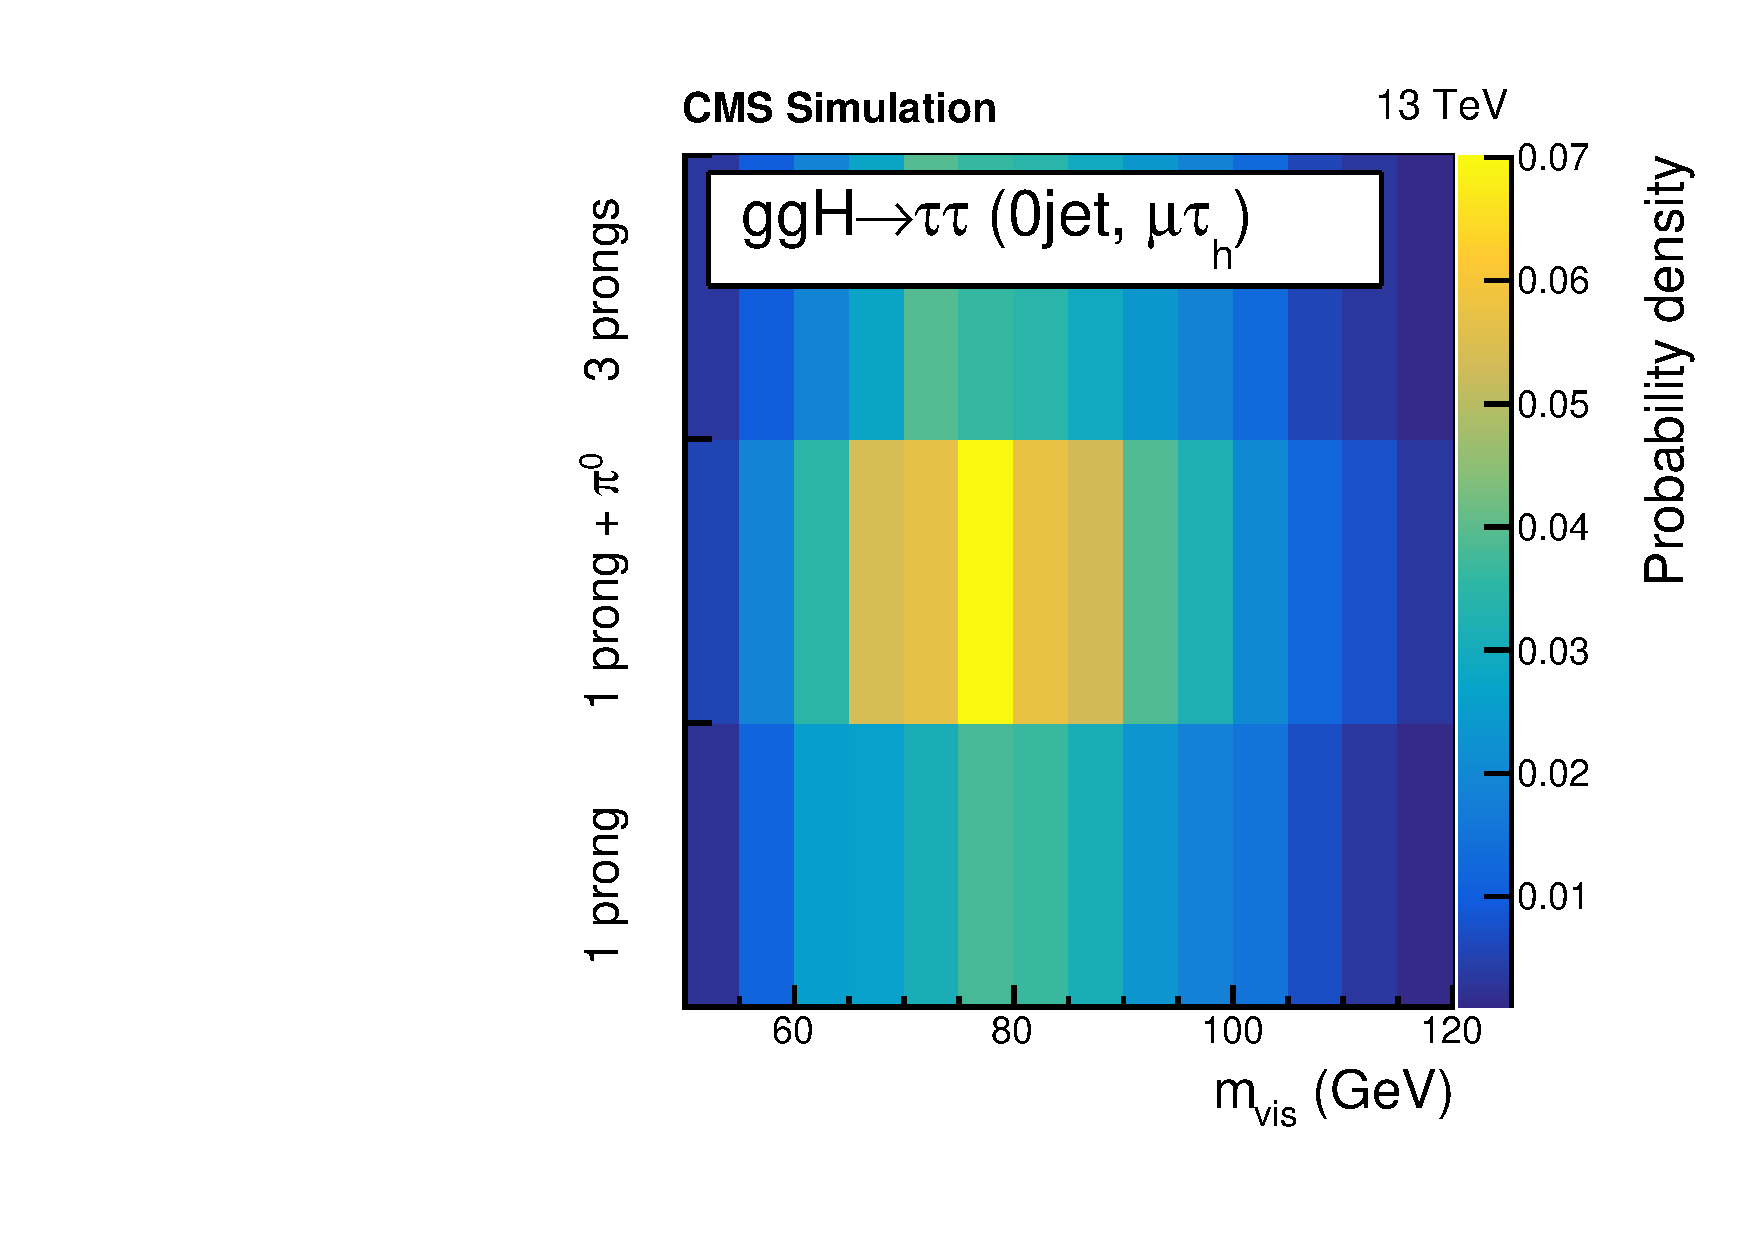
\includegraphics[width=0.4\textwidth]{figures/Figure_001-a.pdf}
     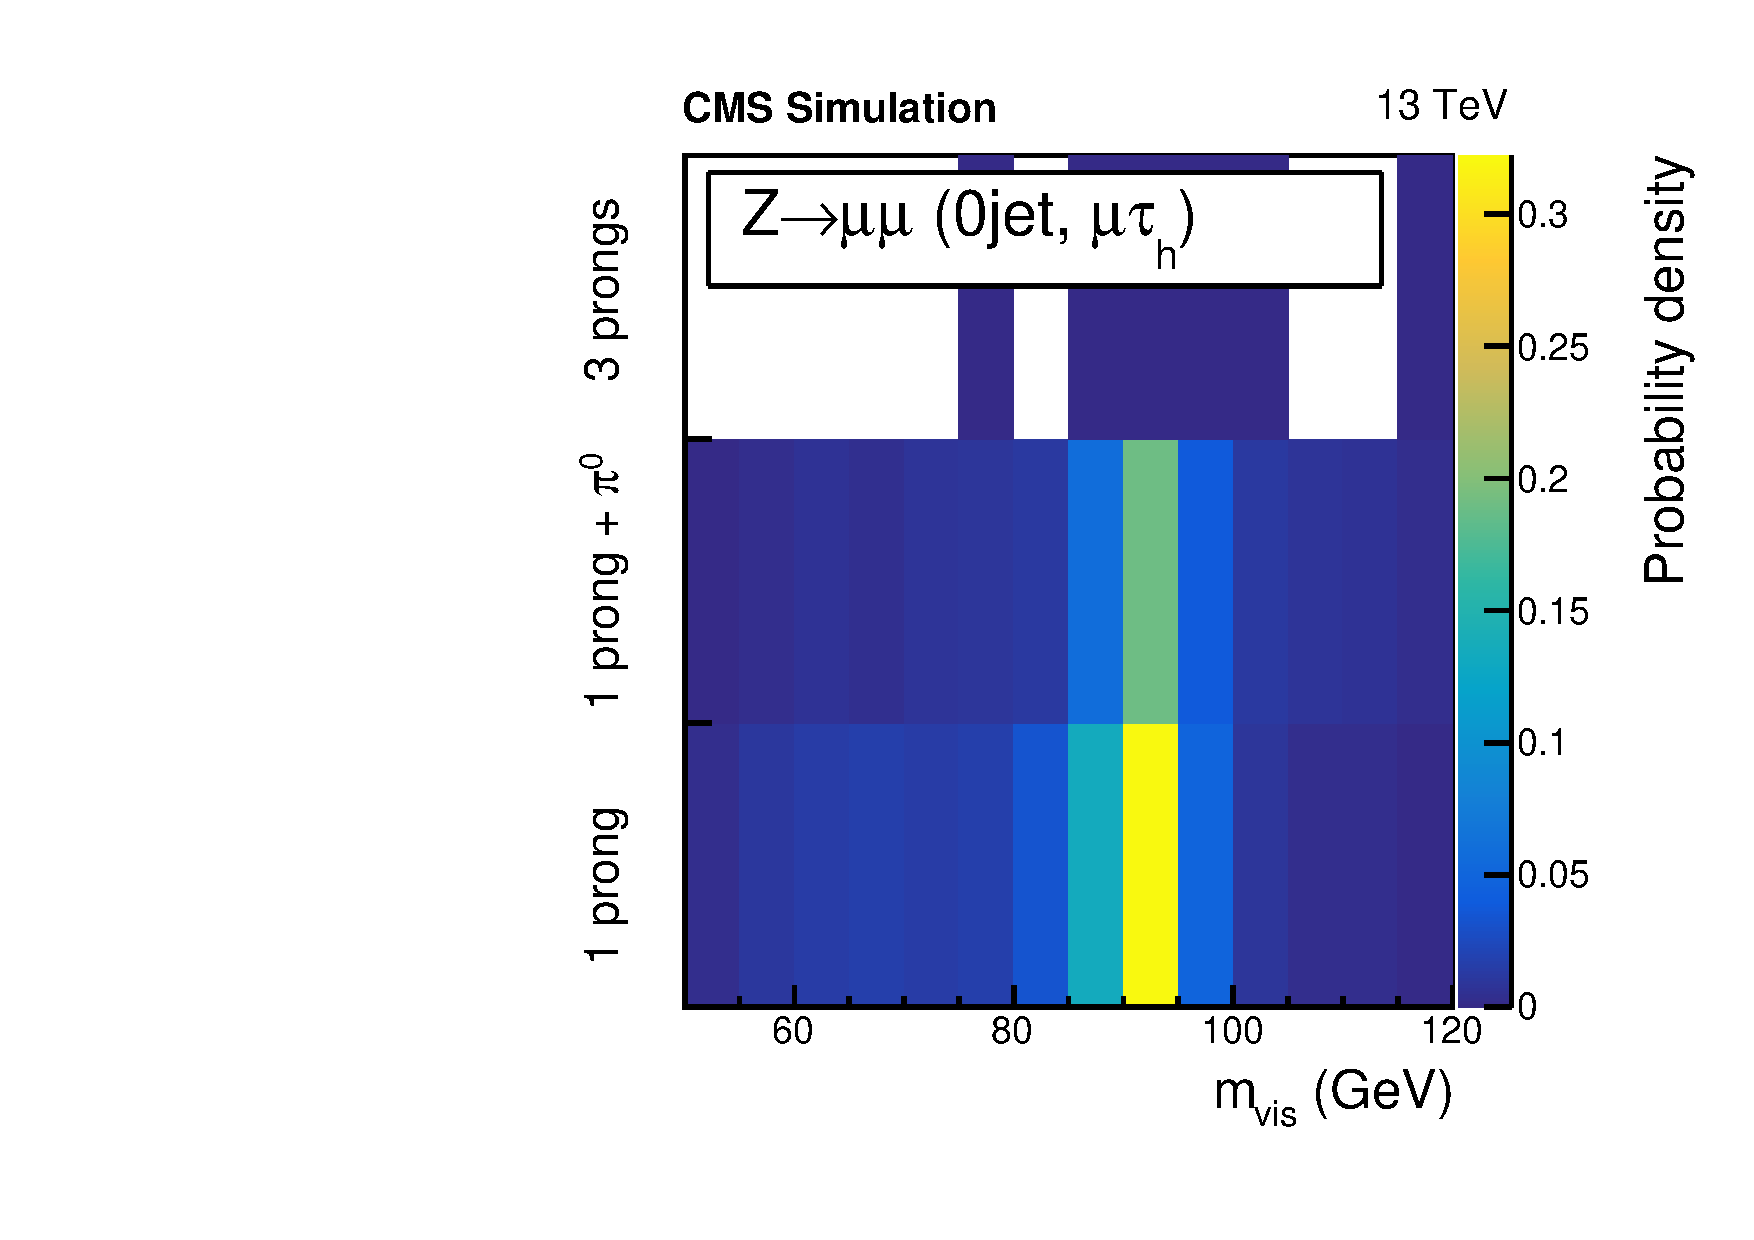
\includegraphics[width=0.4\textwidth]{figures/Figure_001-b.pdf}\\
     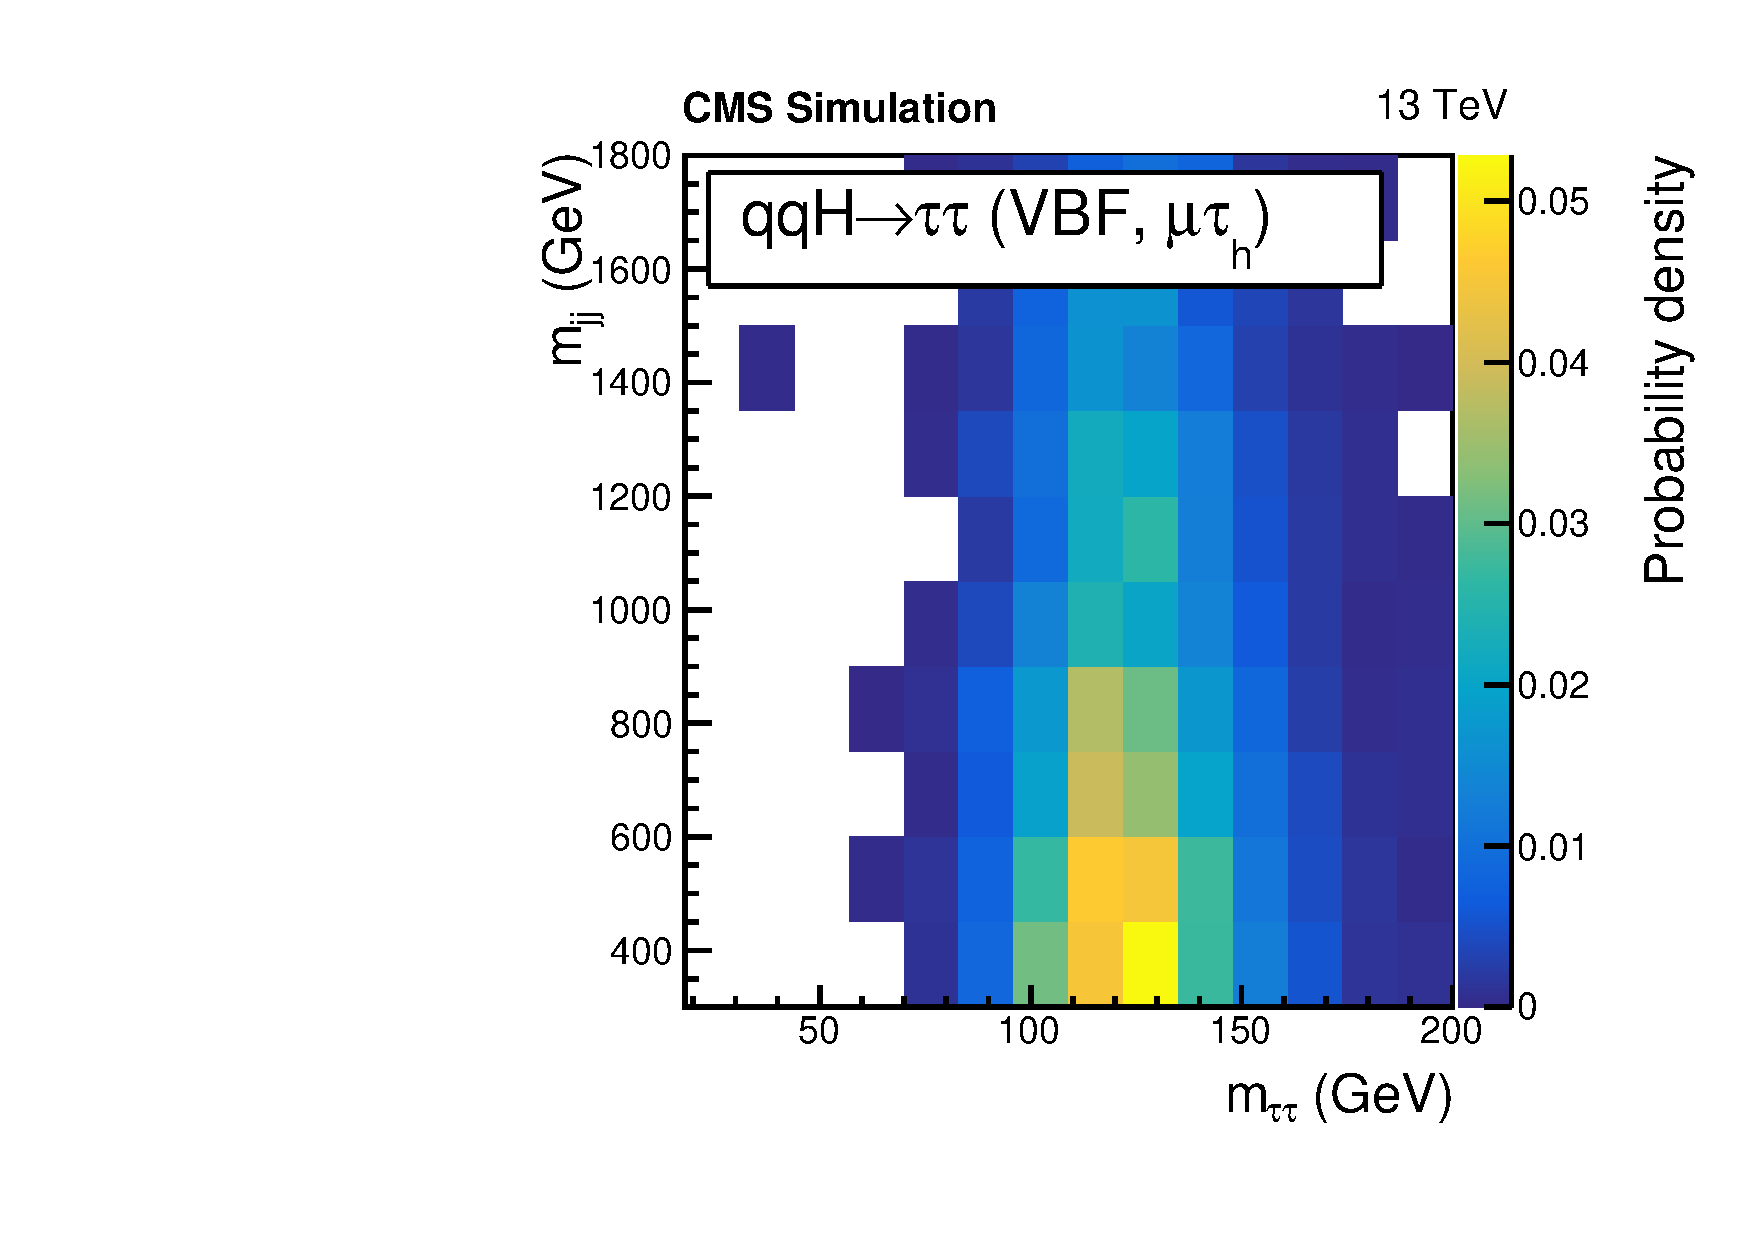
\includegraphics[width=0.4\textwidth]{figures/Figure_001-c.pdf}
     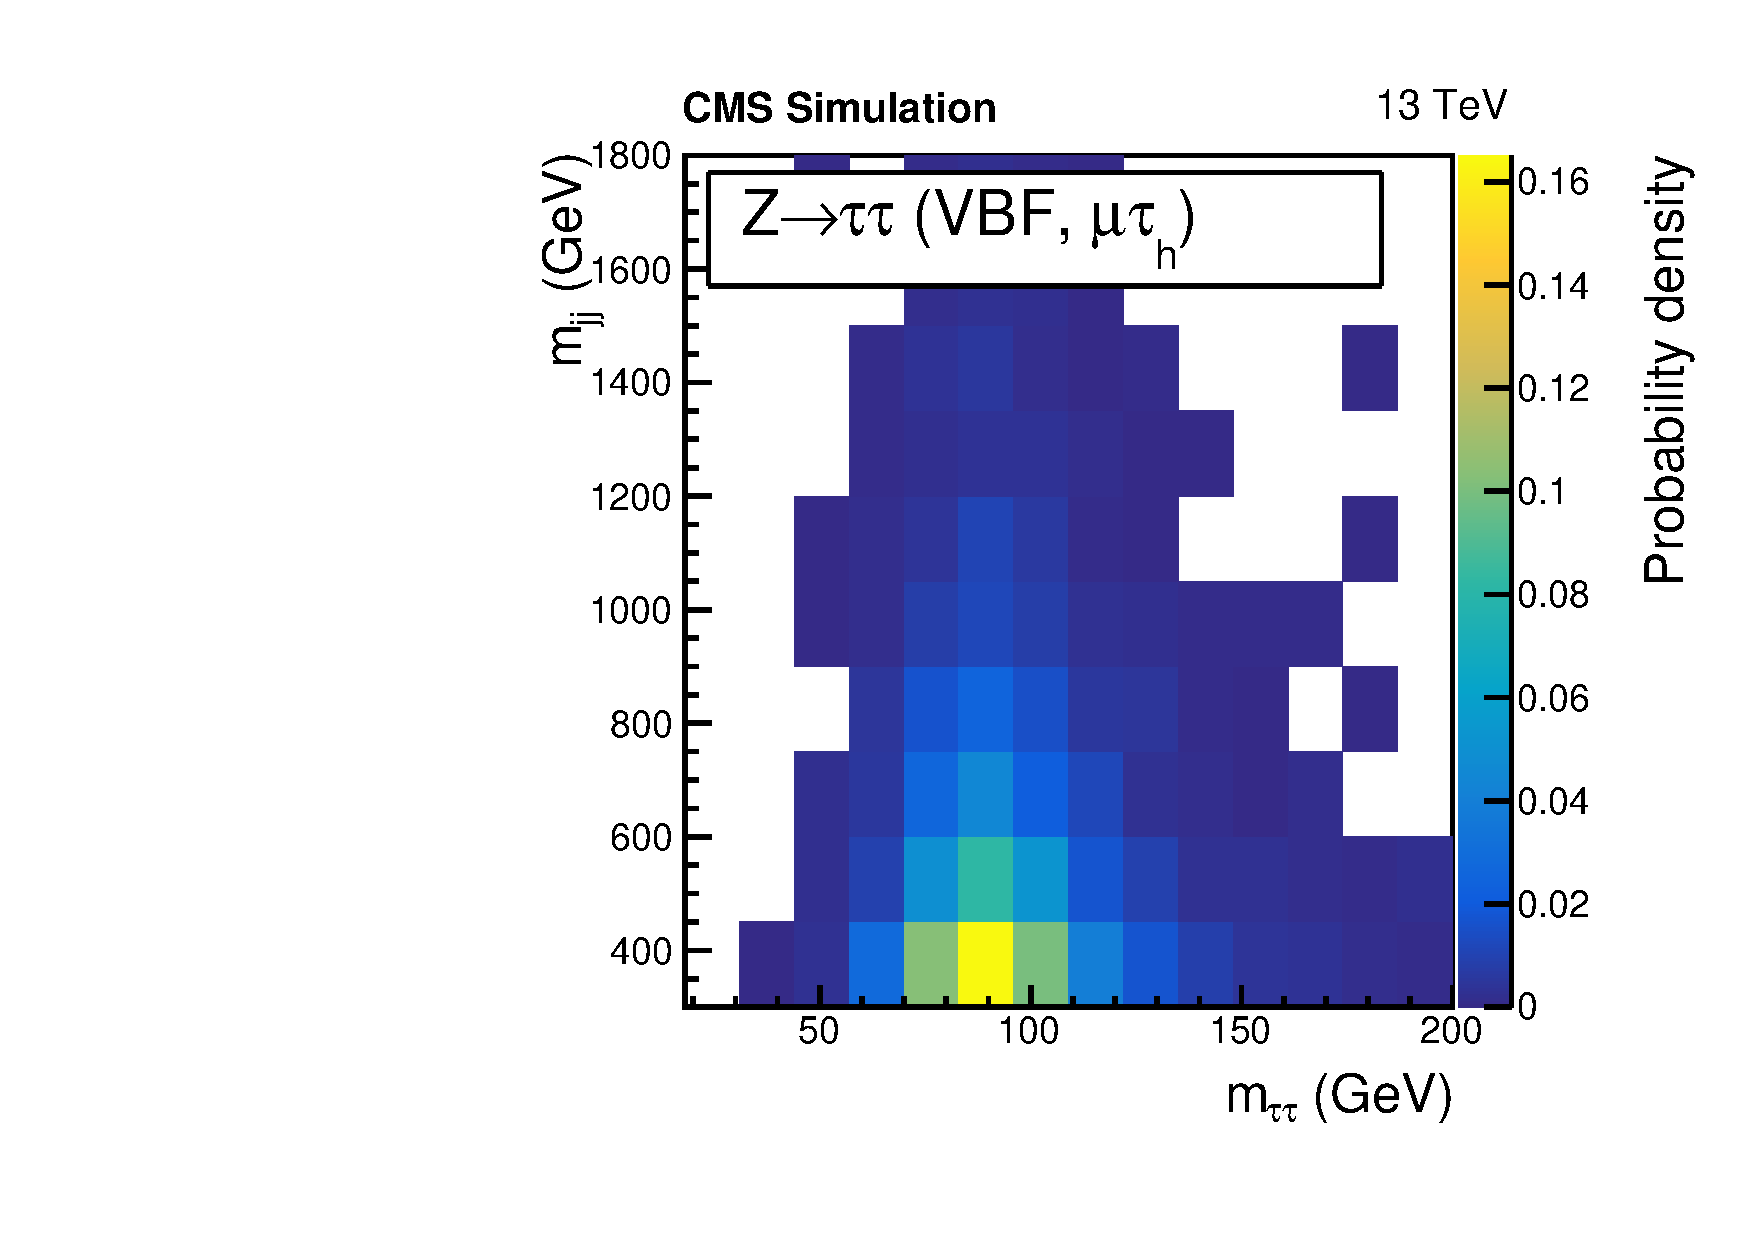
\includegraphics[width=0.4\textwidth]{figures/Figure_001-d.pdf}\\
     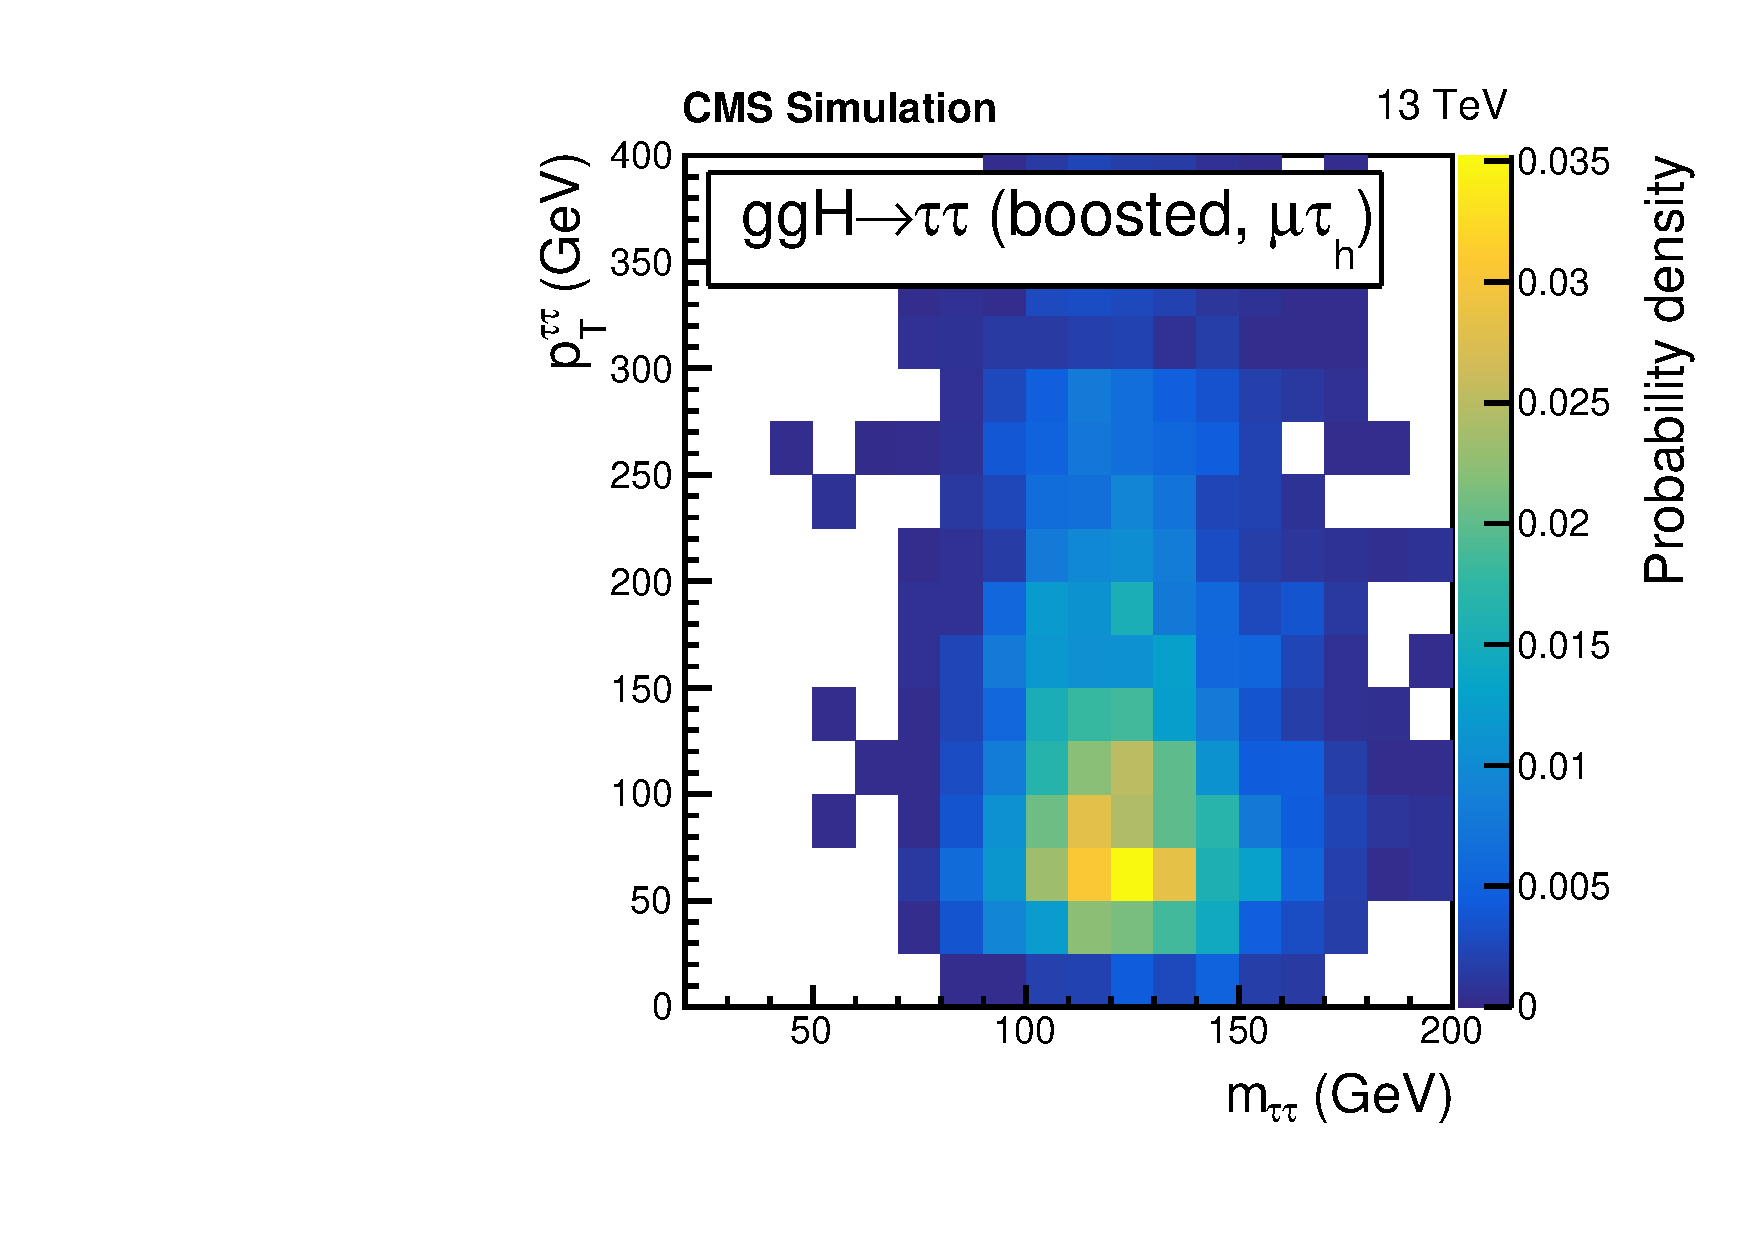
\includegraphics[width=0.4\textwidth]{figures/Figure_001-e.pdf}
     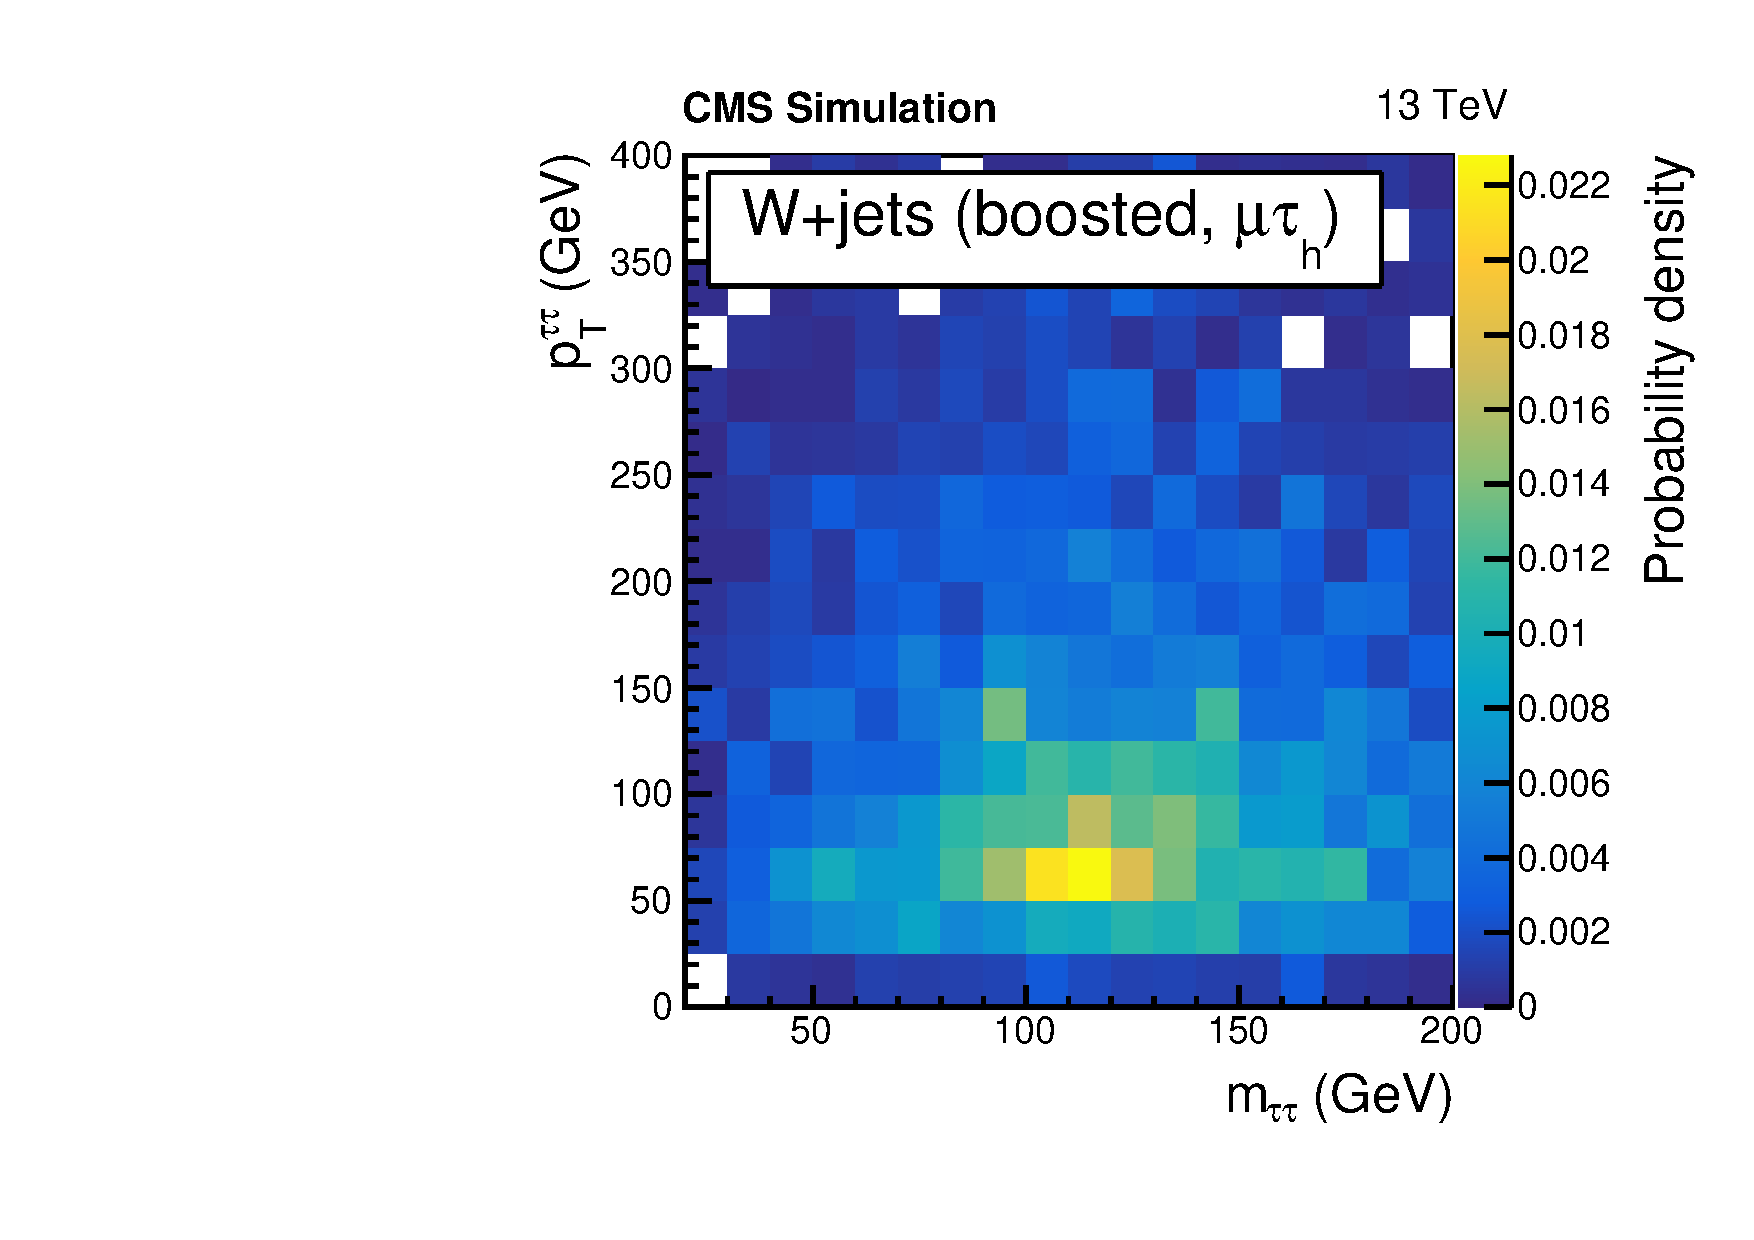
\includegraphics[width=0.4\textwidth]{figures/Figure_001-f.pdf}
     \caption{Distributions for the signal (left) and for some dominant background processes (right) of the two observables chosen in the 0-jet (top), VBF (center), and boosted
(bottom) categories in the $\Pgm\tauh$ decay channel. The background processes are chosen for illustrative purpose for their separation from the signal. The $\PZ\to\Pgm\Pgm$ background in the 0-jet category is concentrated in the regions where the visible mass is close to 90\GeV and is negligible when the $\tauh$ candidate is reconstructed in the 3-prong decay mode. The $\PZ\to\Pgt\Pgt$ background in the VBF category mostly lies at low $\mjj$ values whereas the distribution of VBF signal events extends to high $\mjj$ values. In the boosted category, the W+jets background, which behaves similarly to the QCD multijet background, is rather flat with respect to $\mtt$, and is concentrated at low $\pth$ values. These distributions are not used as such to extract the results.}
     \label{fig:2Dcategories}
\end{figure*}


\begin{table*}
\centering
\begin{tabular}{llll}
 & 0-jet & VBF & Boosted \\
\hline
 & \multicolumn{3}{c}{Selection} \\ \cline{2-4}
$\tauh\tauh$ & No jet &  $\geq$2 jets, $\pth>100\GeV$, $\Delta\eta_{\mathrm{jj}}>2.5$ & Others\\
$\Pgm\tauh$ & No jet &  $\geq$2 jets, $\mjj>300\GeV$, $\pth>50\GeV$, $\pt^{\tauh}>40\GeV$ & Others\\
$\Pe\tauh$ & No jet &  $\geq$2 jets, $\mjj>300\GeV$, $\pth>50\GeV$ & Others\\
$\Pe\Pgm$ & No jet & 2 jets, $\mjj>300\GeV$ & Others \\
\hline
 & \multicolumn{3}{c}{Observables}\\ \cline{2-4}
$\tauh\tauh$ & $\mtt$                 &    $\mjj$, $\mtt$  &   $\pth$, $\mtt$  \\
$\Pgm\tauh$ & $\tauh$ decay mode, $\mvis$   &    $\mjj$, $\mtt$  &  $\pth$, $\mtt$  \\
$\Pe\tauh$ & $\tauh$ decay mode, $\mvis$   &    $\mjj$, $\mtt$  &  $\pth$, $\mtt$ \\
$\Pe\Pgm$ & $\pt^{\Pgm}$, $\mvis$   &     $\mjj$, $\mtt$  &   $\pth$, $\mtt$  \\
\hline
\end{tabular}
\caption{ Category selection and observables used to build the 2D kinematic distributions. The events neither selected in the 0-jet nor in the VBF category are included in the boosted category, as denoted by ``Others".
\label{tab:categories}
}
\end{table*}

\subsection{Channels}
\section{Data Set}
\section{MC Samples}
\section{Triggers}
\section{SVFit Algorithm}
\section{Background Estimation}
The largest irreducible source of background is the Drell--Yan production
of $\PZ/\Pgg^*\to\Pgt\Pgt, \ell\ell$.
In order to correct the yield and distributions of the $\PZ/\Pgg^*\to\Pgt\Pgt, \ell\ell$ simulations to better reproduce the Drell--Yan process in data, a dedicated control sample of $\PZ/\Pgg^*\to\Pgm\Pgm$
events is collected in data with a single-muon trigger, and compared to simulation. The control sample is composed of events with two well-identified
and well-isolated opposite-charge muons with $\pt$ greater than 25\GeV and an invariant mass between 70 and 110\GeV.
More than 99\% of events in this region come from $\PZ/\Pgg^*\to\Pgm\Pgm$ decays.
Differences in the distributions of $m_{\ell\ell/\Pgt\Pgt}$ and $\pt(\ell\ell/\Pgt\Pgt)$ in data and in simulations are observed in this control region, and 2D weights based on these variables are derived and applied to simulated $\PZ/\Pgg^*\to\Pgt\Pgt, \ell\ell$ events in the signal region of the analysis. In addition, corrections depending on $\mjj$ are derived from the $\PZ/\Pgg^*\to\Pgm\Pgm$ region and applied to the $\PZ/\Pgg^*\to\Pgt\Pgt, \ell\ell$ simulation for events with at least two jets passing the VBF category selection criteria. After this reweighting, good agreement between data in the $\PZ/\Pgg^*\to\Pgm\Pgm$ region and simulation is found for all other variables.
The simulated sample is split, on the basis of the matching between objects at the generator and at the detector levels,
into events with prompt leptons (muons or electrons), hadronic decays of the $\Pgt$ leptons,
and jets or misidentified objects at the detector level that do not have corresponding objects
at generator level within $\Delta R < 0.2$.
The electroweak production of $\PZ$ bosons in association with two jets is also taken into account in the analysis; it
contributes up to 8\% of the $\PZ$ boson production in the VBF category.

The background from $\PW+\text{jets}$ production contributes significantly to the
$\Pgm\tauh$ and $\Pe\tauh$ channels, when the $\PW$ boson decays leptonically and
a jet is misidentified as a $\tauh$ candidate.
The $\PW+\text{jets}$ distributions are modelled using simulation, while their yields are estimated using data, as detailed below. In the boosted and VBF categories, statistical fluctuations in the distributions from simulations are reduced by relaxing the isolation of the $\tauh$ and $\ell$ candidates, which has been checked not to bias the distributions.
The simulated sample is normalized in such a way as to obtain agreement between the yields in data and the predicted backgrounds in a control region enriched in the $\PW+\text{jets}$ background,
which is obtained by applying all selection criteria,
with the exception that $\MT$ is required to be greater than 80\GeV instead of less than 50\GeV.
The $\PW+\text{jets}$ event purity in this
region varies from about 50\% in the boosted category to 85\% in the 0-jet category.
The high-$\MT$ sidebands described above, for each category, are considered
as a control regions in this fit.
 The constraints obtained in the boosted category are extrapolated to the VBF category of the corresponding decay channel because
the topology of the boosted and VBF events is similar, and few data events would pass the high-$\MT$ sideband selection in the VBF category. Figure~\ref{fig:CR1} shows the control regions with $\MT>80$\GeV in the 0-jet and boosted categories of the $\Pgm\tauh$ and $\Pe\tauh$ channels. These control regions are composed of only one bin because they are used solely to constrain the normalization of the $\PW+\text{jets}$ process.
In the $\Pe\Pgm$ and $\tauh\tauh$ decay channels, the $\PW+\text{jets}$
background is small compared to other backgrounds, and its contribution is
estimated from simulations.

\begin{figure*}[!htbp]
\centering
     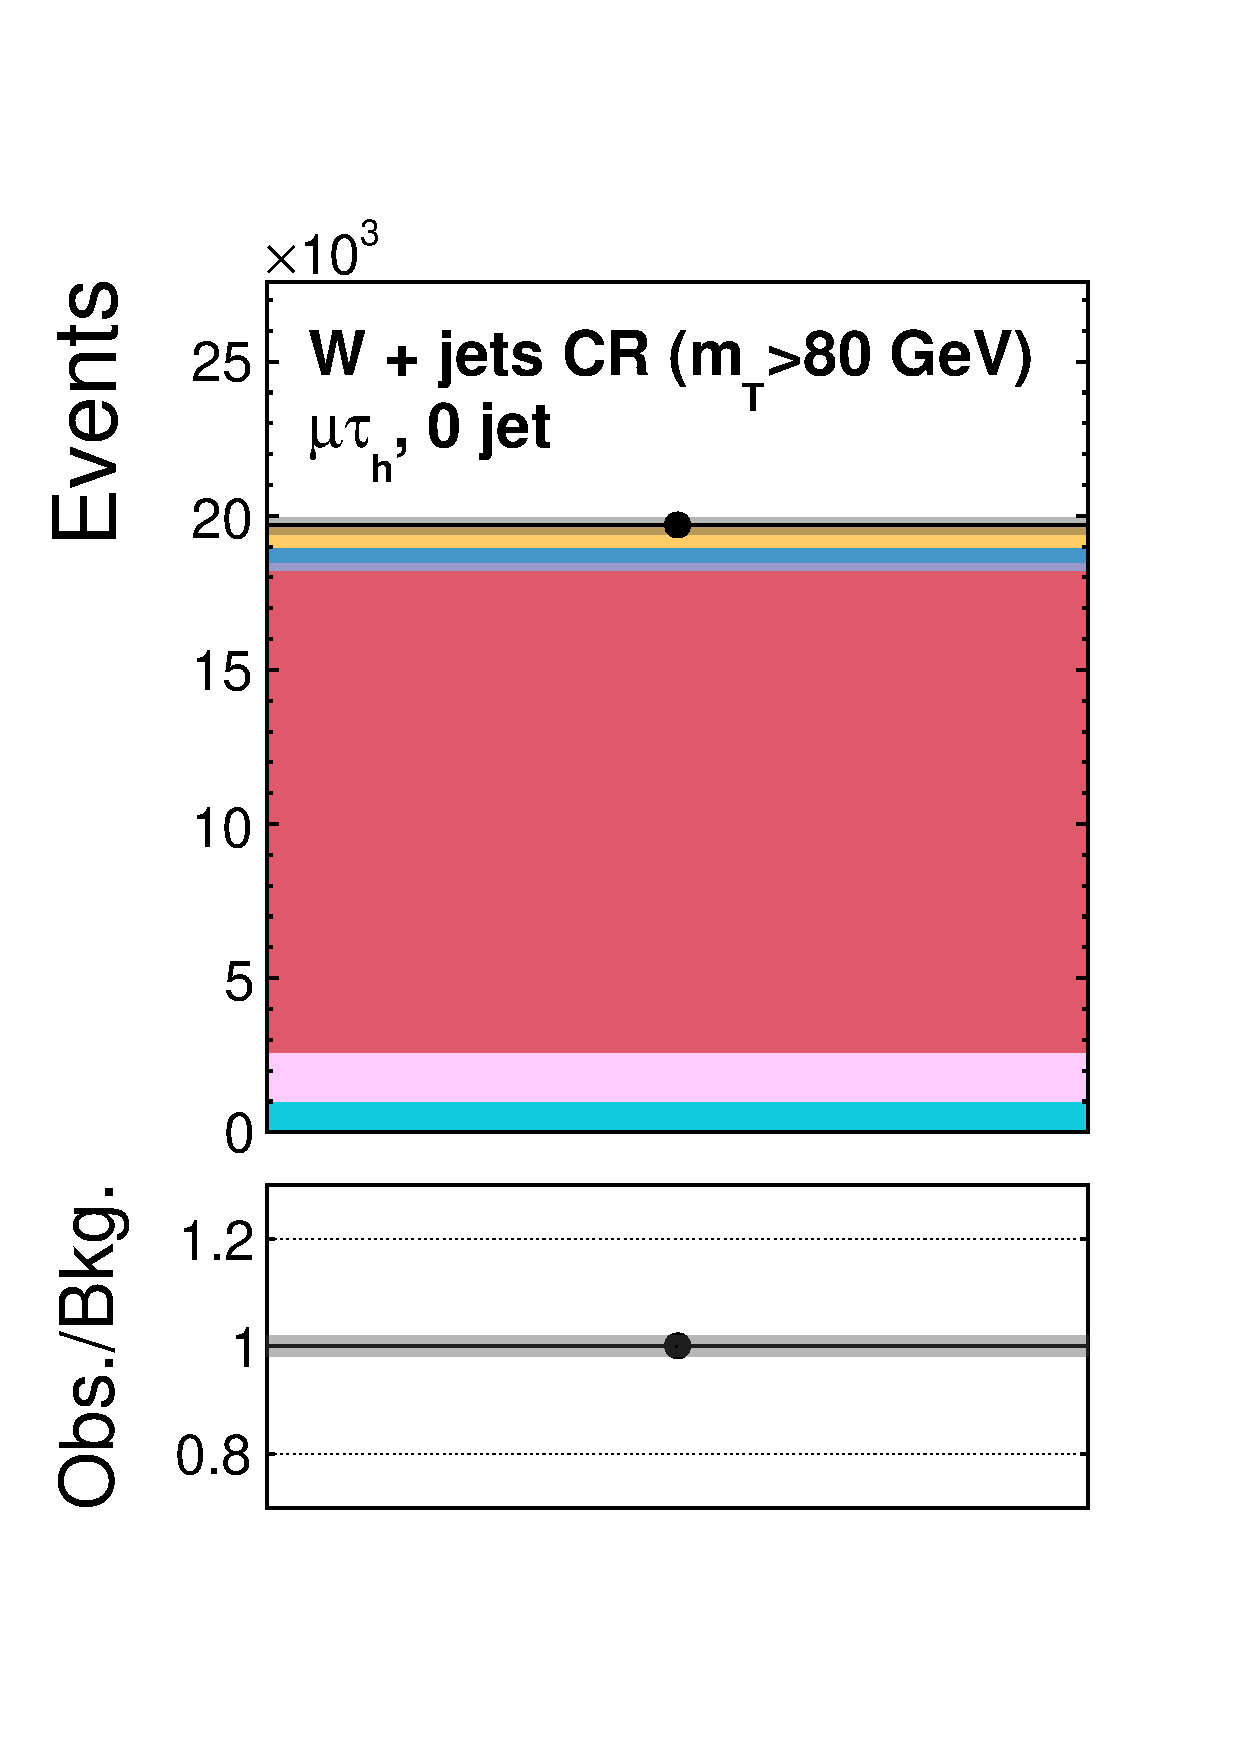
\includegraphics[width=0.19\textwidth]{figures/Figure_002-a.pdf}
     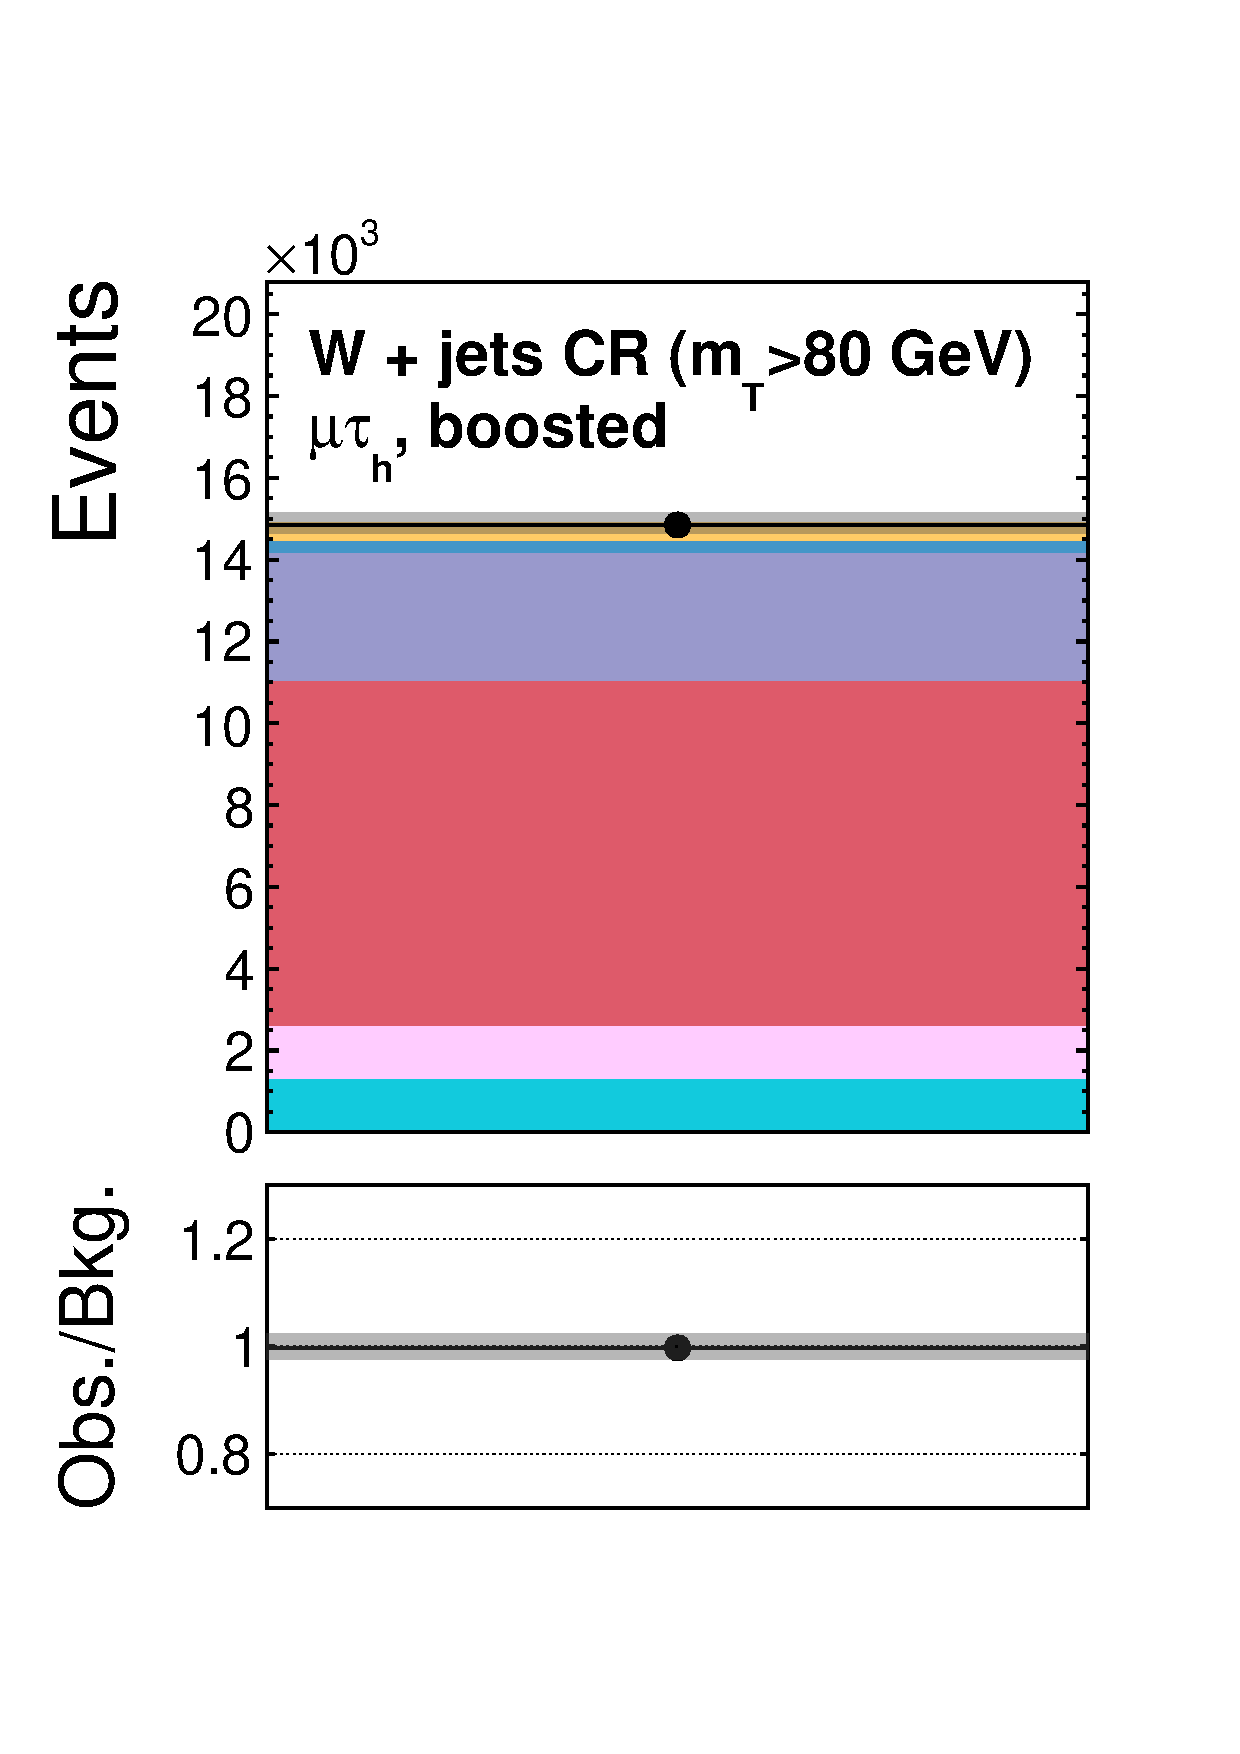
\includegraphics[width=0.19\textwidth]{figures/Figure_002-b.pdf}
     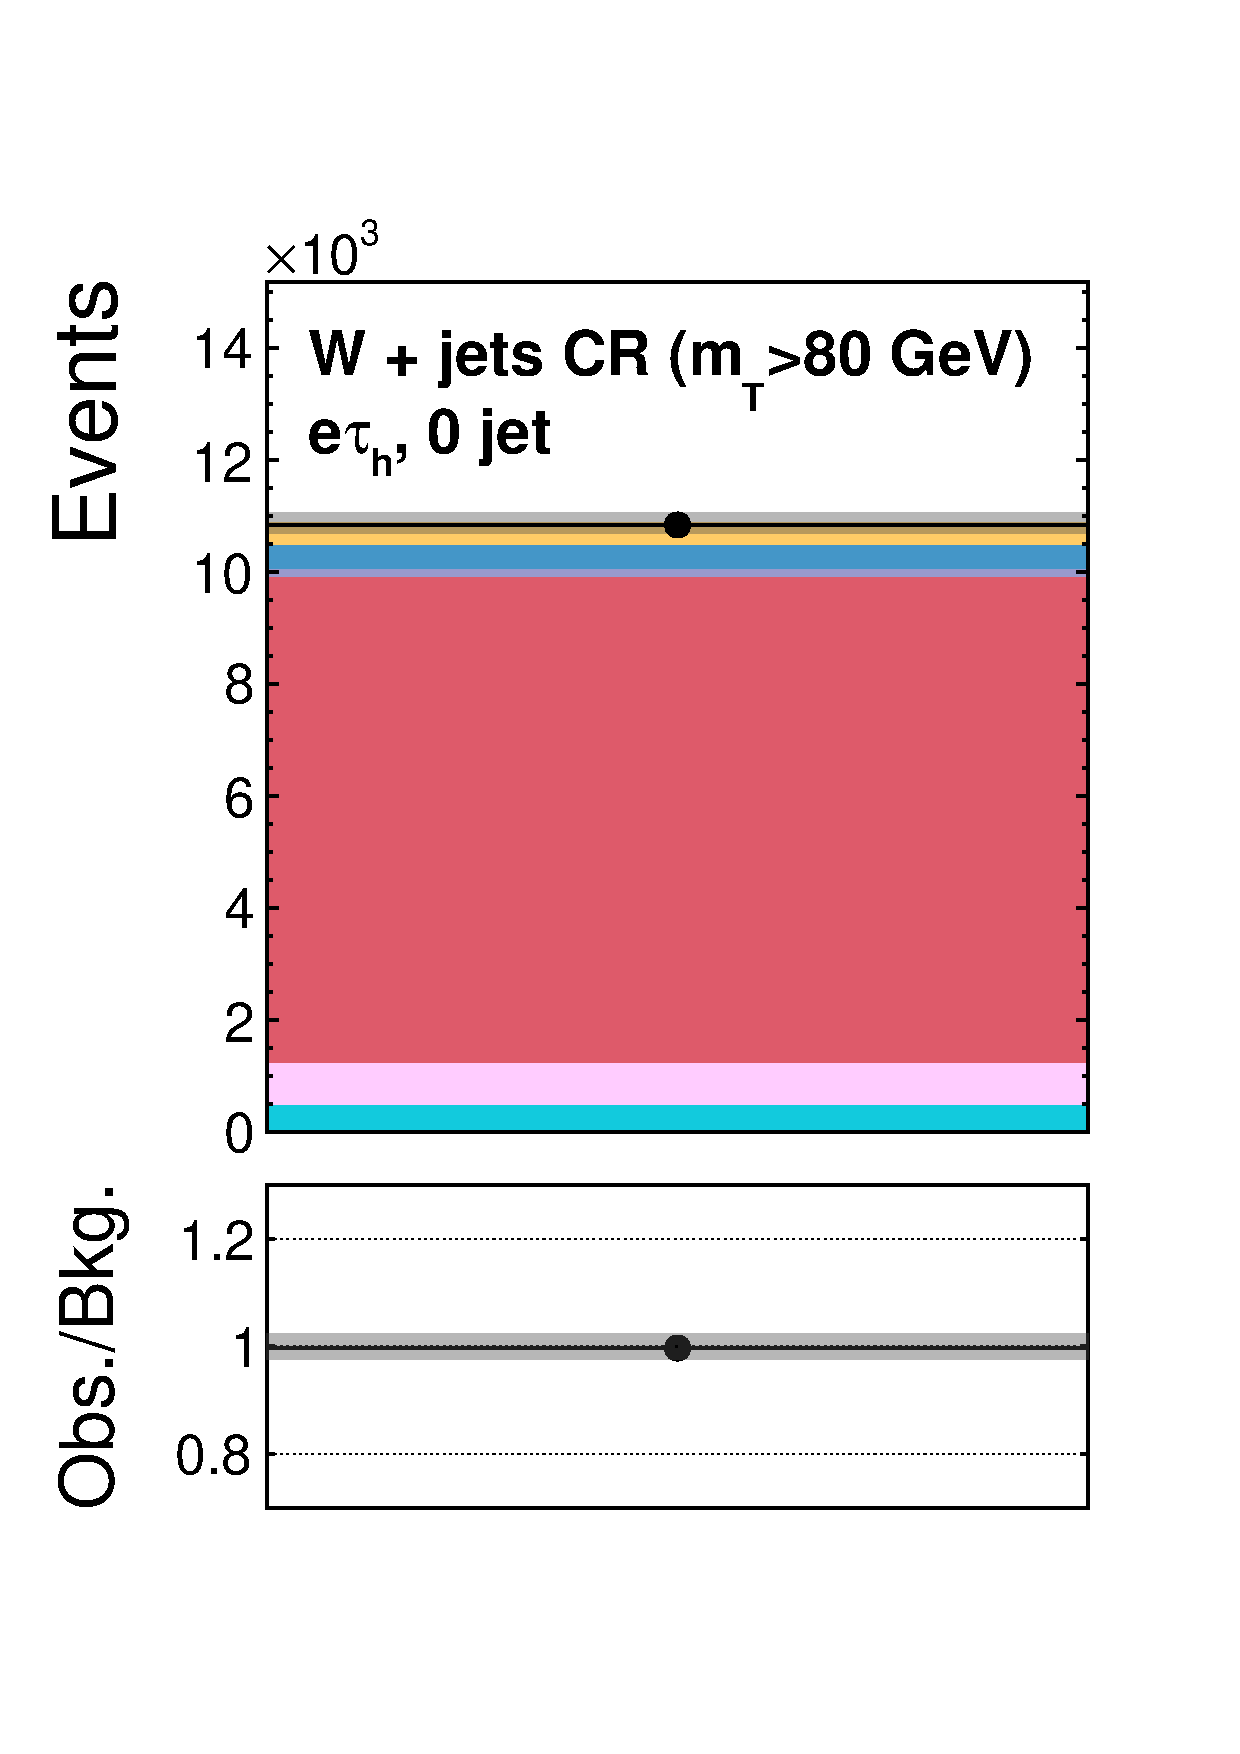
\includegraphics[width=0.19\textwidth]{figures/Figure_002-c.pdf}
     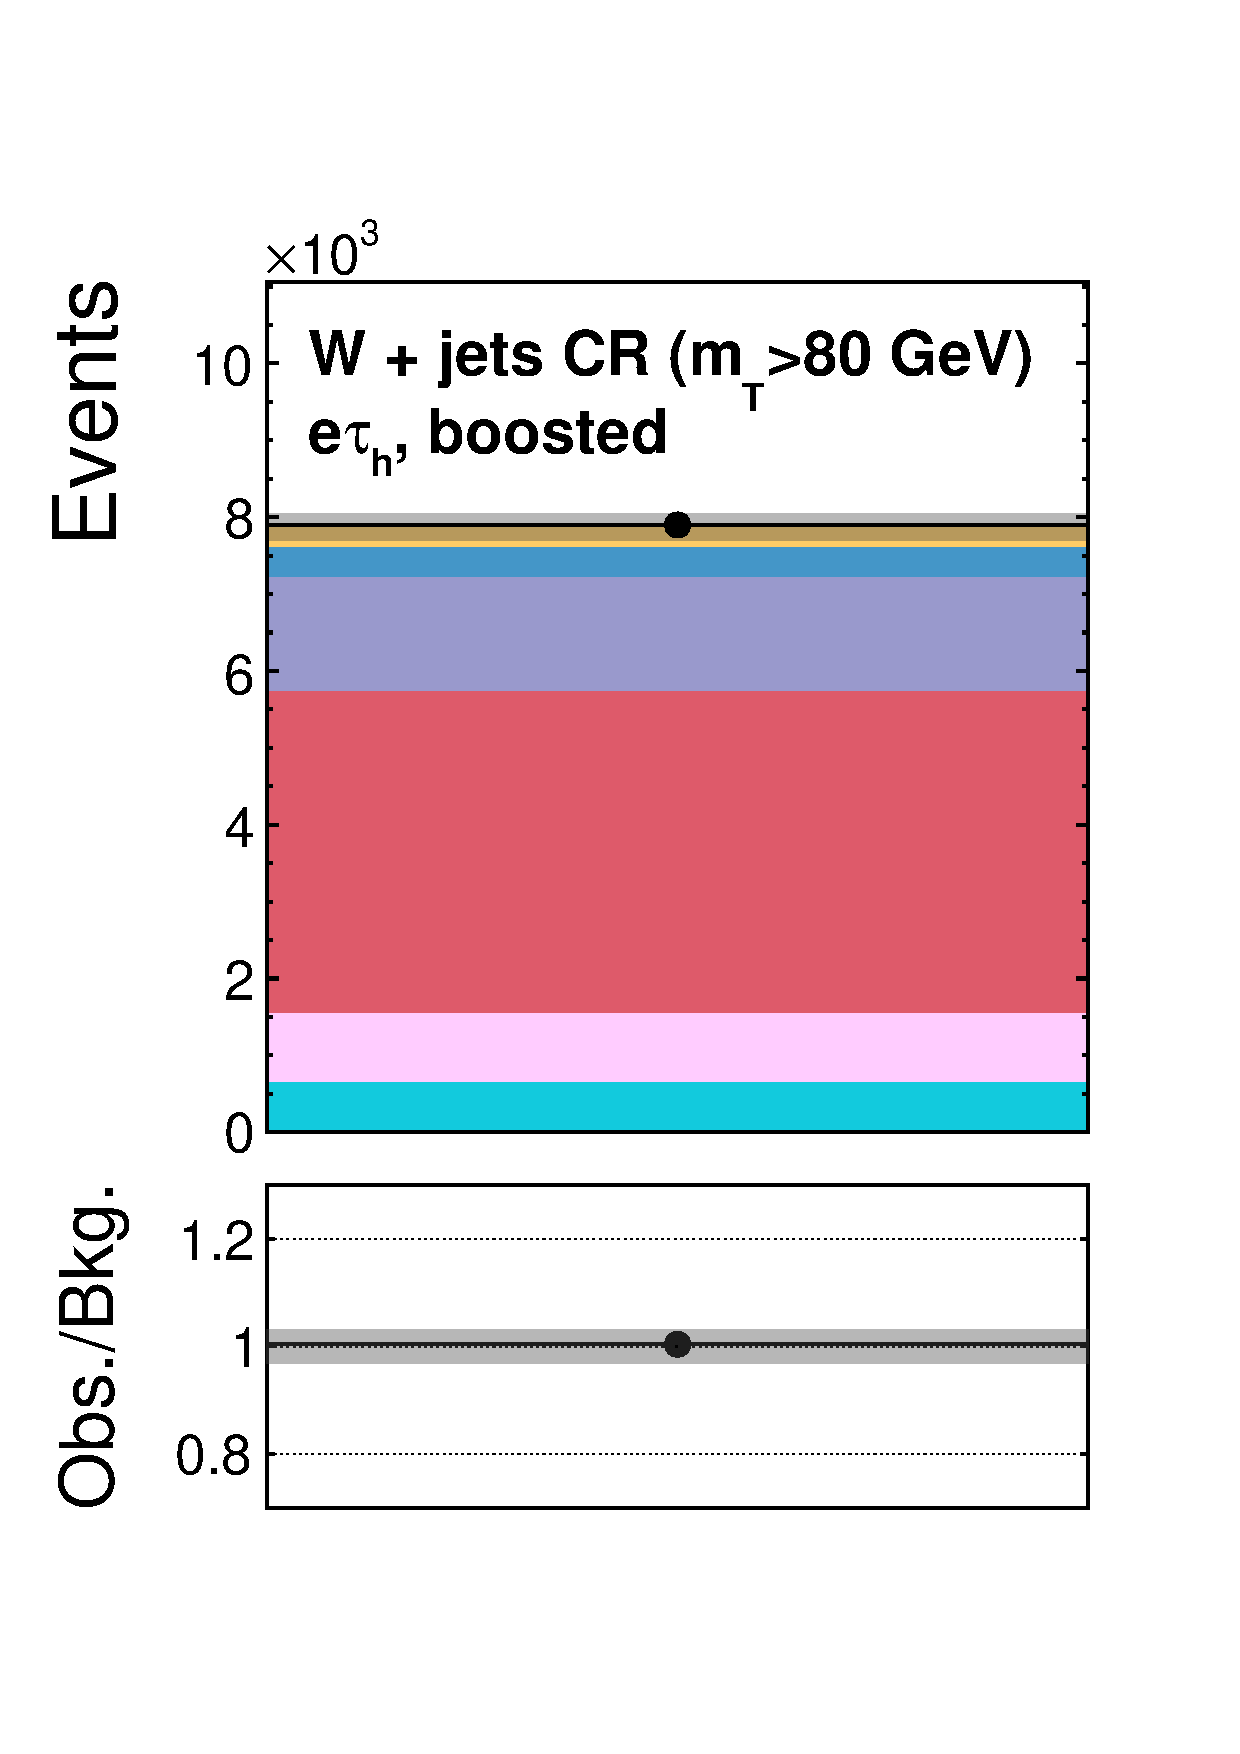
\includegraphics[width=0.19\textwidth]{figures/Figure_002-d.pdf}
     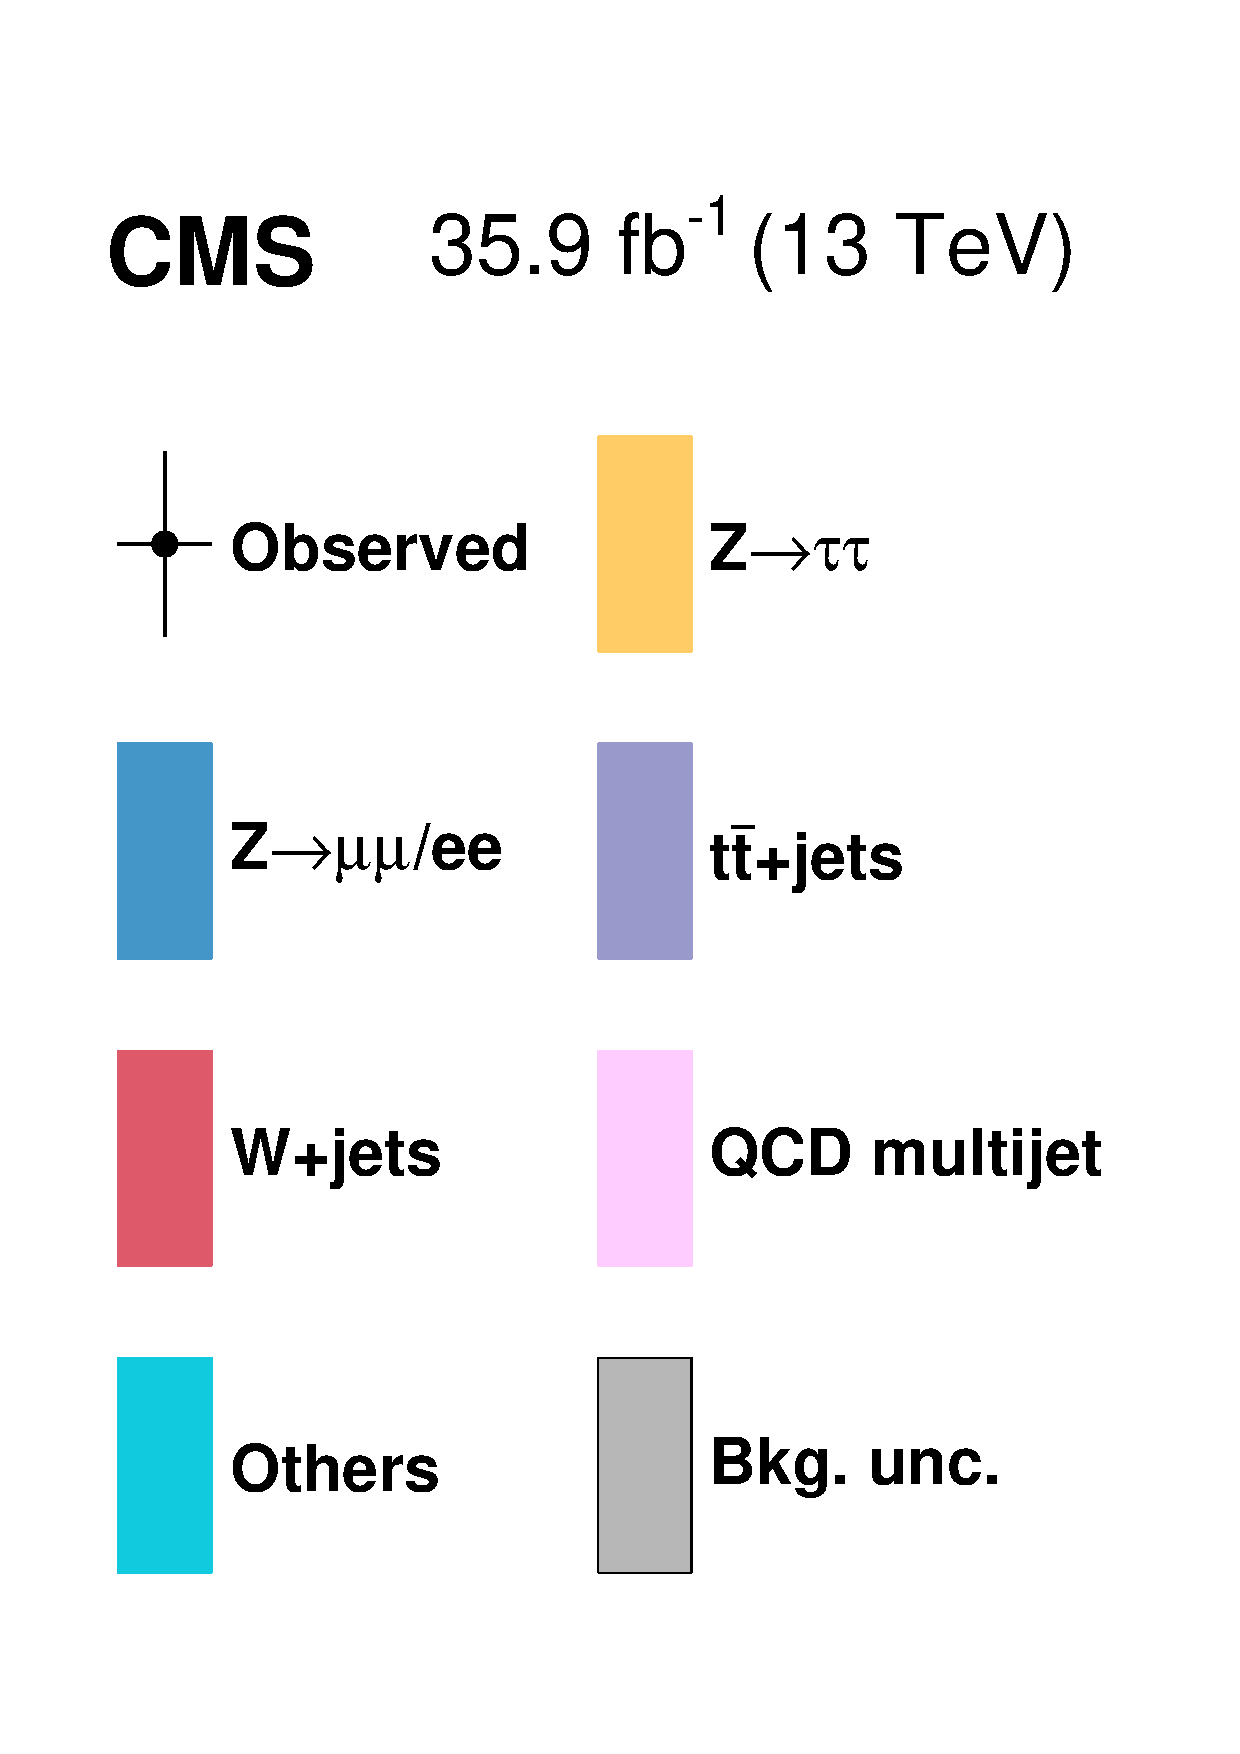
\includegraphics[width=0.19\textwidth]{figures/Figure_002-e.pdf}
     \caption{Control regions enriched in the $\PW+\text{jets}$ background used in the maximum likelihood fit, together with the signal regions, to extract the results. The normalization of the predicted background distributions corresponds to the result of the global fit. These regions, defined with $\MT>80$\GeV,  control the
yields of the $\PW+\text{jets}$ background in the $\Pgm\tauh$ and $\Pe\tauh$ channels.  The constraints obtained in the boosted categories are propagated to the VBF categories of the corresponding channels.}
     \label{fig:CR1}
\end{figure*}


The QCD multijet events constitute another important source of reducible background in the $\ell \tauh$ channels, and it is entirely estimated from data. Various control samples are constituted to estimate the shape and the yield of the QCD multijet background in these channels, as explained below:
\begin{enumerate}
\item The raw yield is extracted using a sample where the
$\ell$ and the $\tauh$ candidates have the same sign. Using this sample, the QCD multijet process is estimated from data by subtracting the contribution of the Drell--Yan, \ttbar, diboson,
and $\PW+\text{jets}$ processes.
\item The yield obtained above is corrected to account for differences between the background composition in the same-sign and opposite-sign regions. The extrapolation factor between the same-sign and opposite-sign regions is determined by comparing the yield of the QCD multijet background for events with $\ell$ candidates passing inverted isolation criteria, in the same-sign and opposite-sign regions. It is constrained and measured by adding to the global fit the opposite-sign region where the $\ell$ candidates pass inverted isolation criteria, using the QCD multijet background estimate from the same-sign region with $\ell$ candidates passing inverted isolation criteria. For the same reasons as in the case of the W+jets background, the constraints are also extrapolated to the VBF signal region. Figure~\ref{fig:CR3} shows these control regions for the 0-jet and boosted categories of the $\Pgm\tauh$ and $\Pe\tauh$ channels; the observable is $\mvis$ or $\mtt$ to provide discrimination between the QCD multijet and the $\PZ\to\Pgt\Pgt$ processes.
\item The 2D distributions of the QCD multijet background are estimated from a region with same-sign leptons, as for the yield estimate, but the isolation of the $\ell$ and $\tauh$ candidates is additionally relaxed to reduce the statistical fluctuations in the distributions. Again the contribution of the Drell--Yan, \ttbar, diboson,
and $\PW+ \text{jets}$ processes are subtracted from data to extract the QCD multijet contribution in this region.
\end{enumerate}
The same technique is used in the $\Pe\Pgm$ decay channel, but no control region is included in the fit because QCD multijet events contribute little to the total background in this decay channel.

\begin{figure*}[!htbp]
\centering
     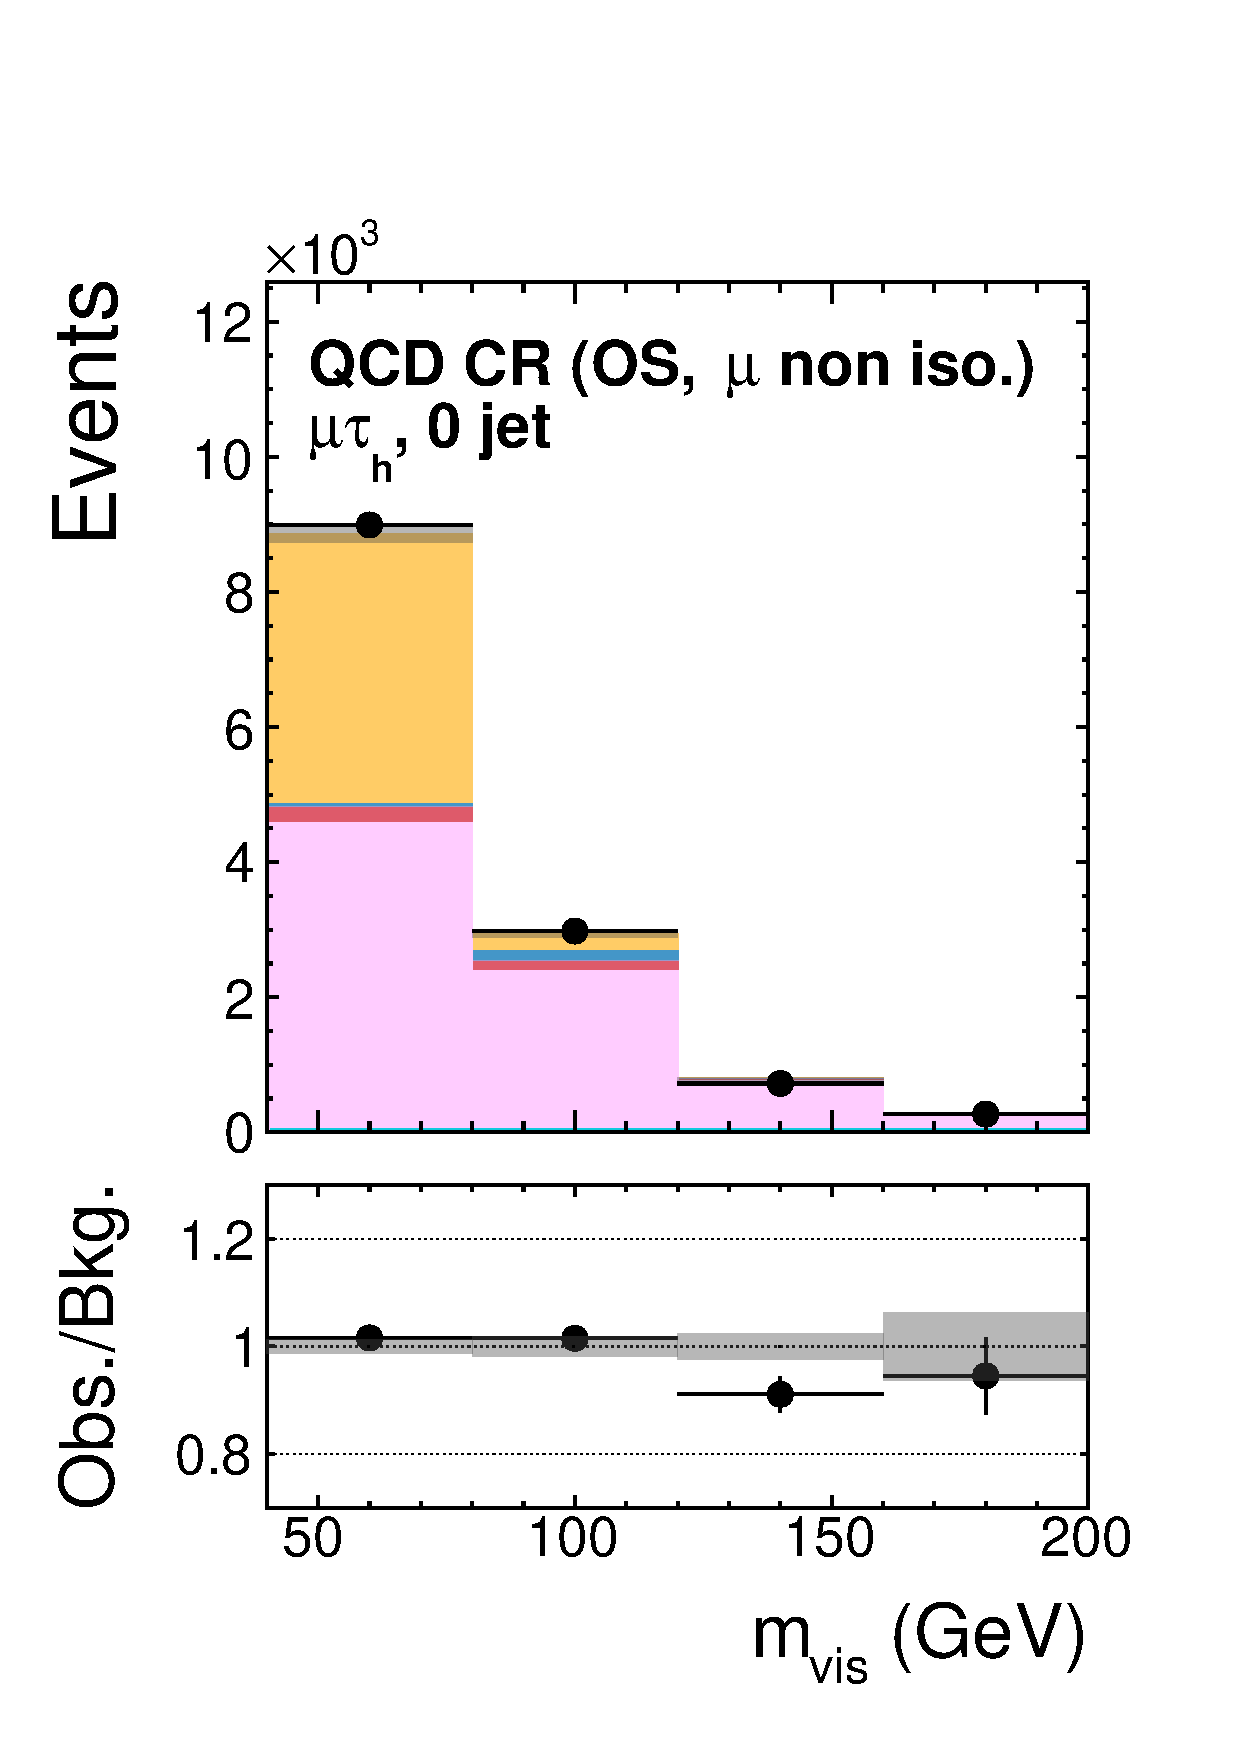
\includegraphics[width=0.3\textwidth]{figures/Figure_003-a.pdf}
     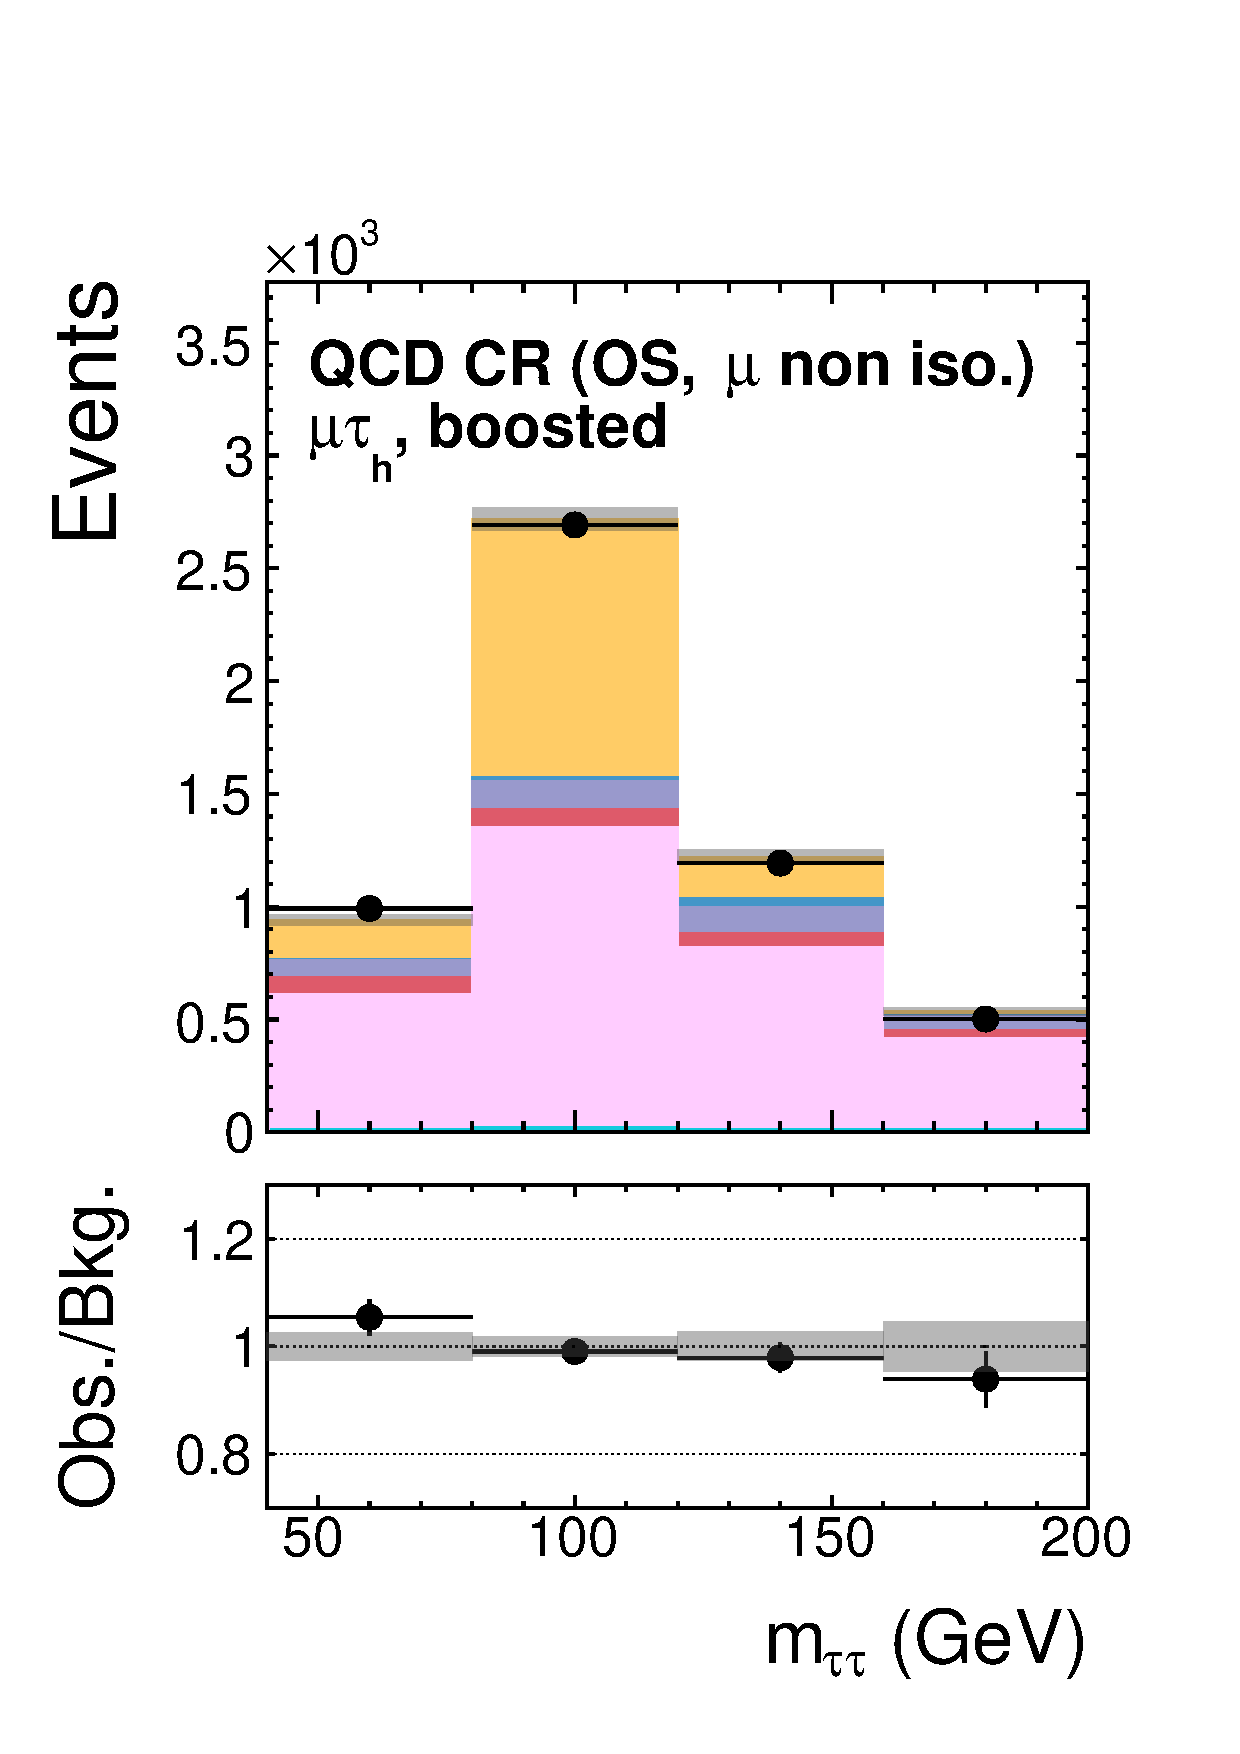
\includegraphics[width=0.3\textwidth]{figures/Figure_003-b.pdf}
     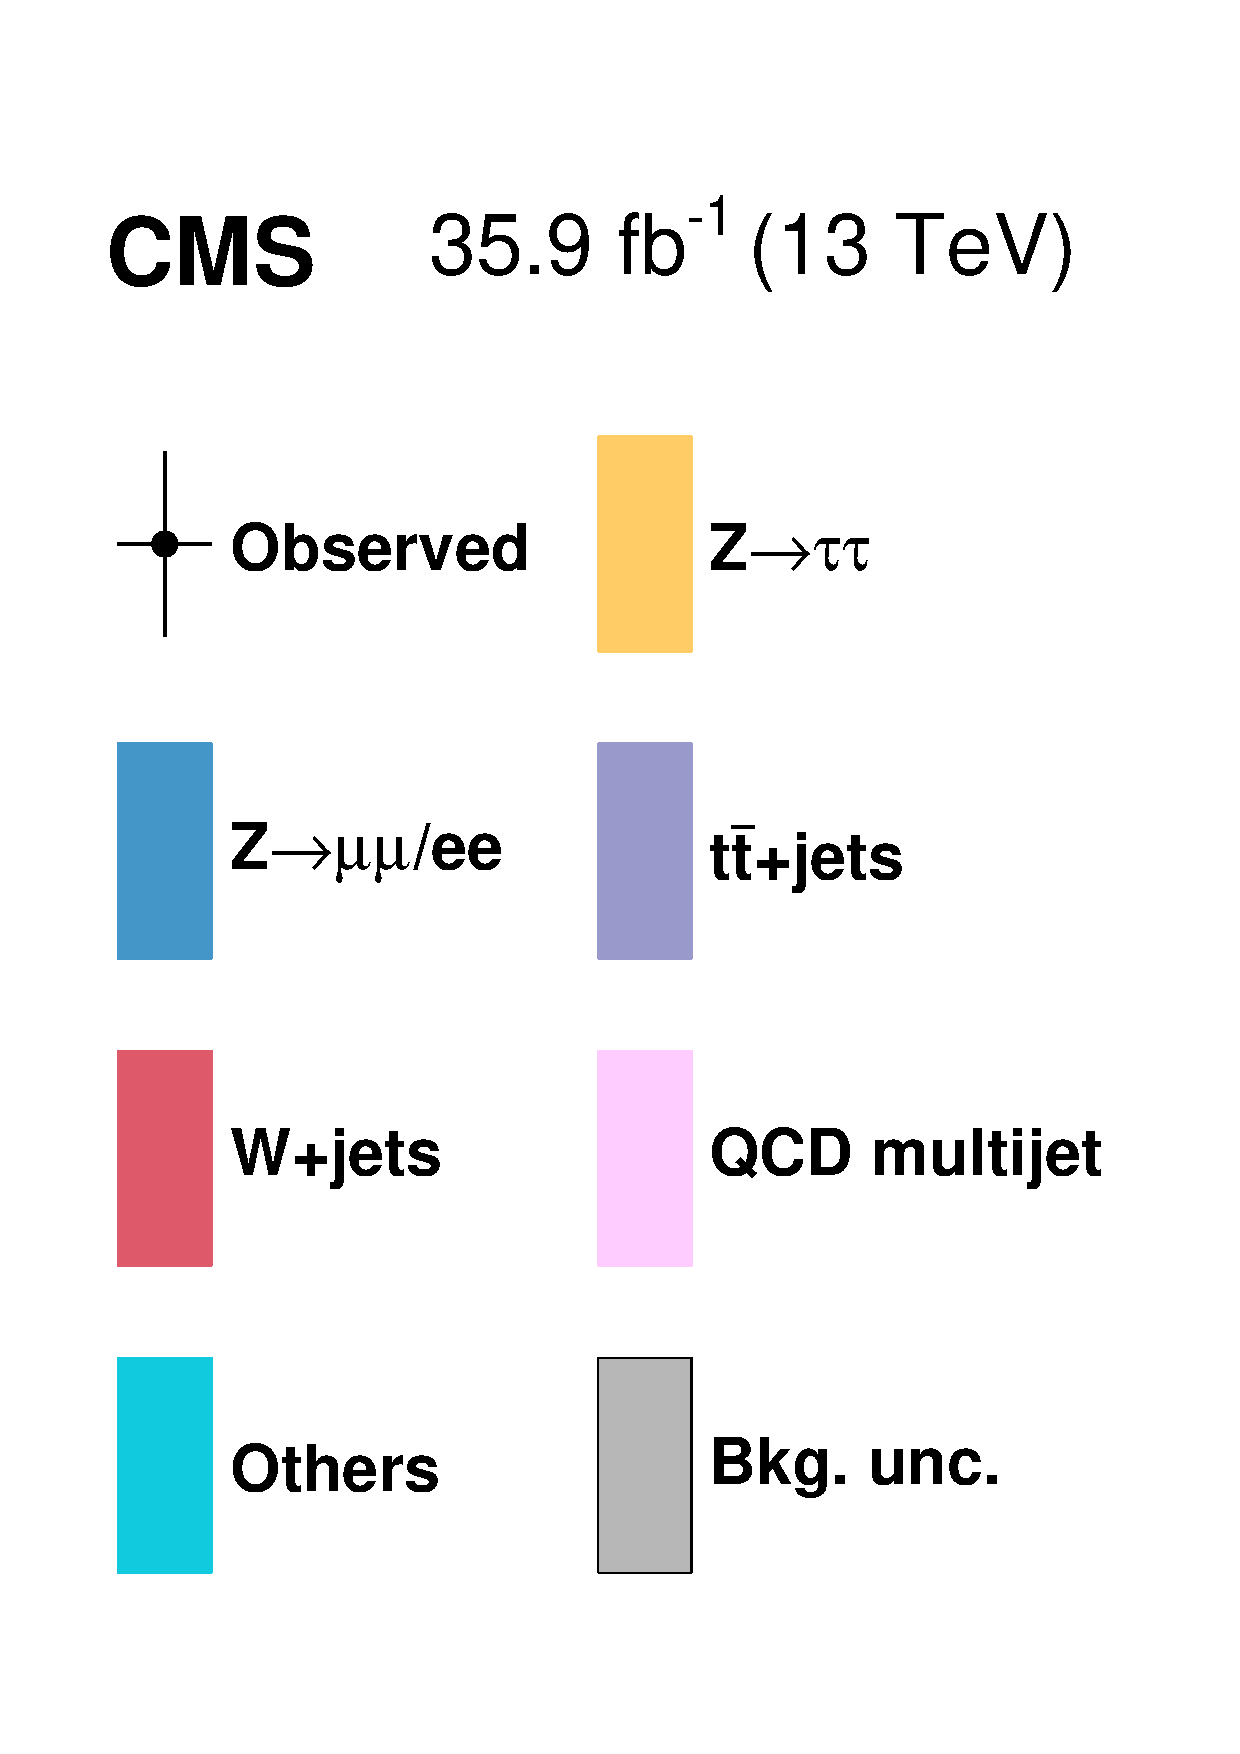
\includegraphics[width=0.3\textwidth]{figures/Figure_003-c.pdf}
     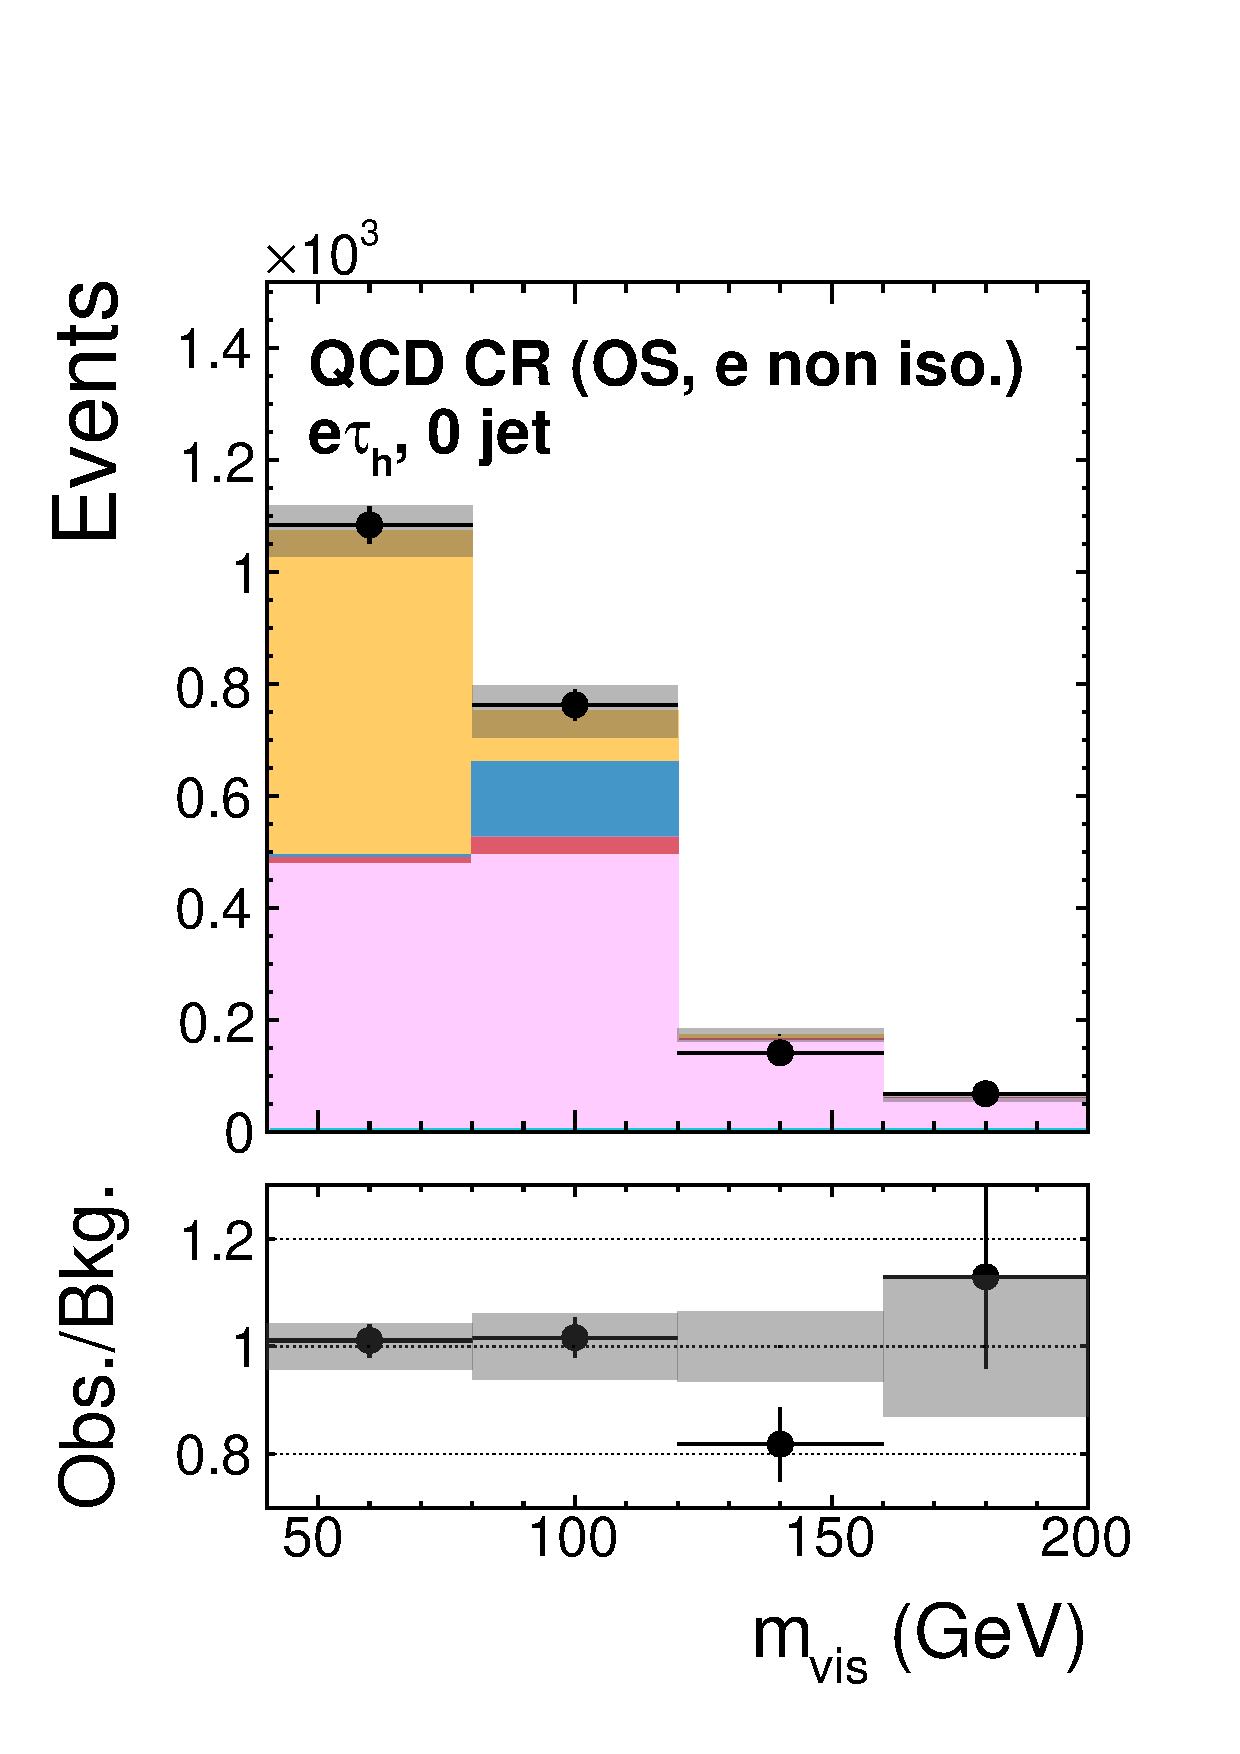
\includegraphics[width=0.3\textwidth]{figures/Figure_003-d.pdf}
     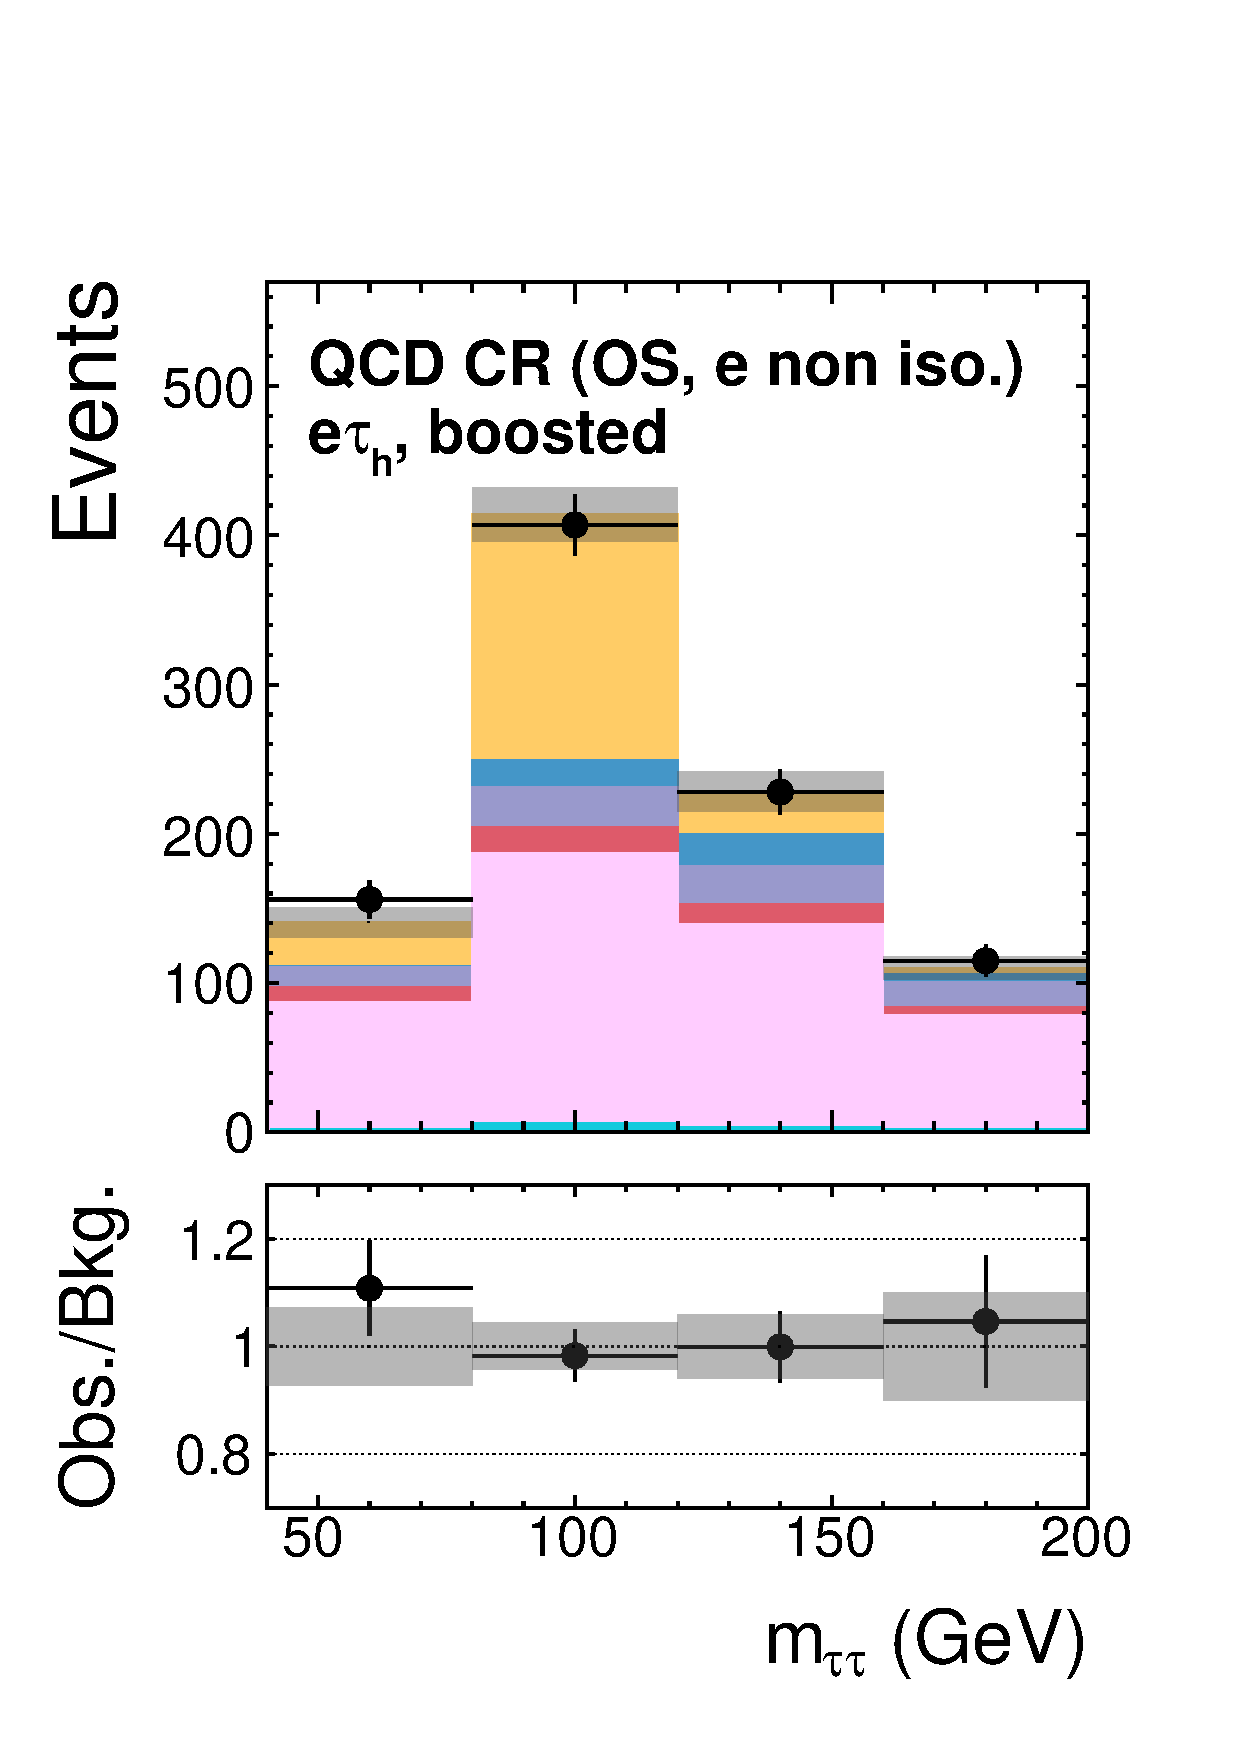
\includegraphics[width=0.3\textwidth]{figures/Figure_003-e.pdf}
     \caption{Control regions enriched in the QCD multijet background used in the maximum likelihood fit, together with the signal regions, to extract the results. The normalization of the predicted background distributions corresponds to the result of the global fit. These regions, defined by selecting events with opposite-sign $\ell$ and $\tauh$ candidates with $\ell$ passing inverted isolation conditions,  control the
yields of the QCD multijet background in the $\Pgm\tauh$ and $\Pe\tauh$ channels.  The constraints obtained in the boosted categories are propagated to the VBF categories of the corresponding channels.}
     \label{fig:CR3}
\end{figure*}

In the $\tauh\tauh$ channel, the large QCD multijet background is estimated with a slightly different method, from
a sample composed of events with opposite-sign $\tauh$ satisfying a relaxed isolation requirement, disjoint from the signal region.
In this region, the QCD multijet background shape and yield are obtained
by subtracting the contribution of the
Drell--Yan, \ttbar, and $\PW+\text{jets}$ processes, estimated as explained above, from the data.
The QCD multijet background yield in the signal region is obtained by multiplying
the yield previously obtained in the control region by an extrapolation factor.
The extrapolation factor is measured in events passing identical selection criteria as those in the signal region, and in the relaxed
isolation region, except that the $\tauh$ candidates are required to have the same sign.
The events selected with opposite-sign $\tauh$ candidates passing relaxed isolation requirements form control regions, shown in Fig.~\ref{fig:CR4}, and are used in the fit to extract the results.

\begin{figure*}[!htbp]
\centering
     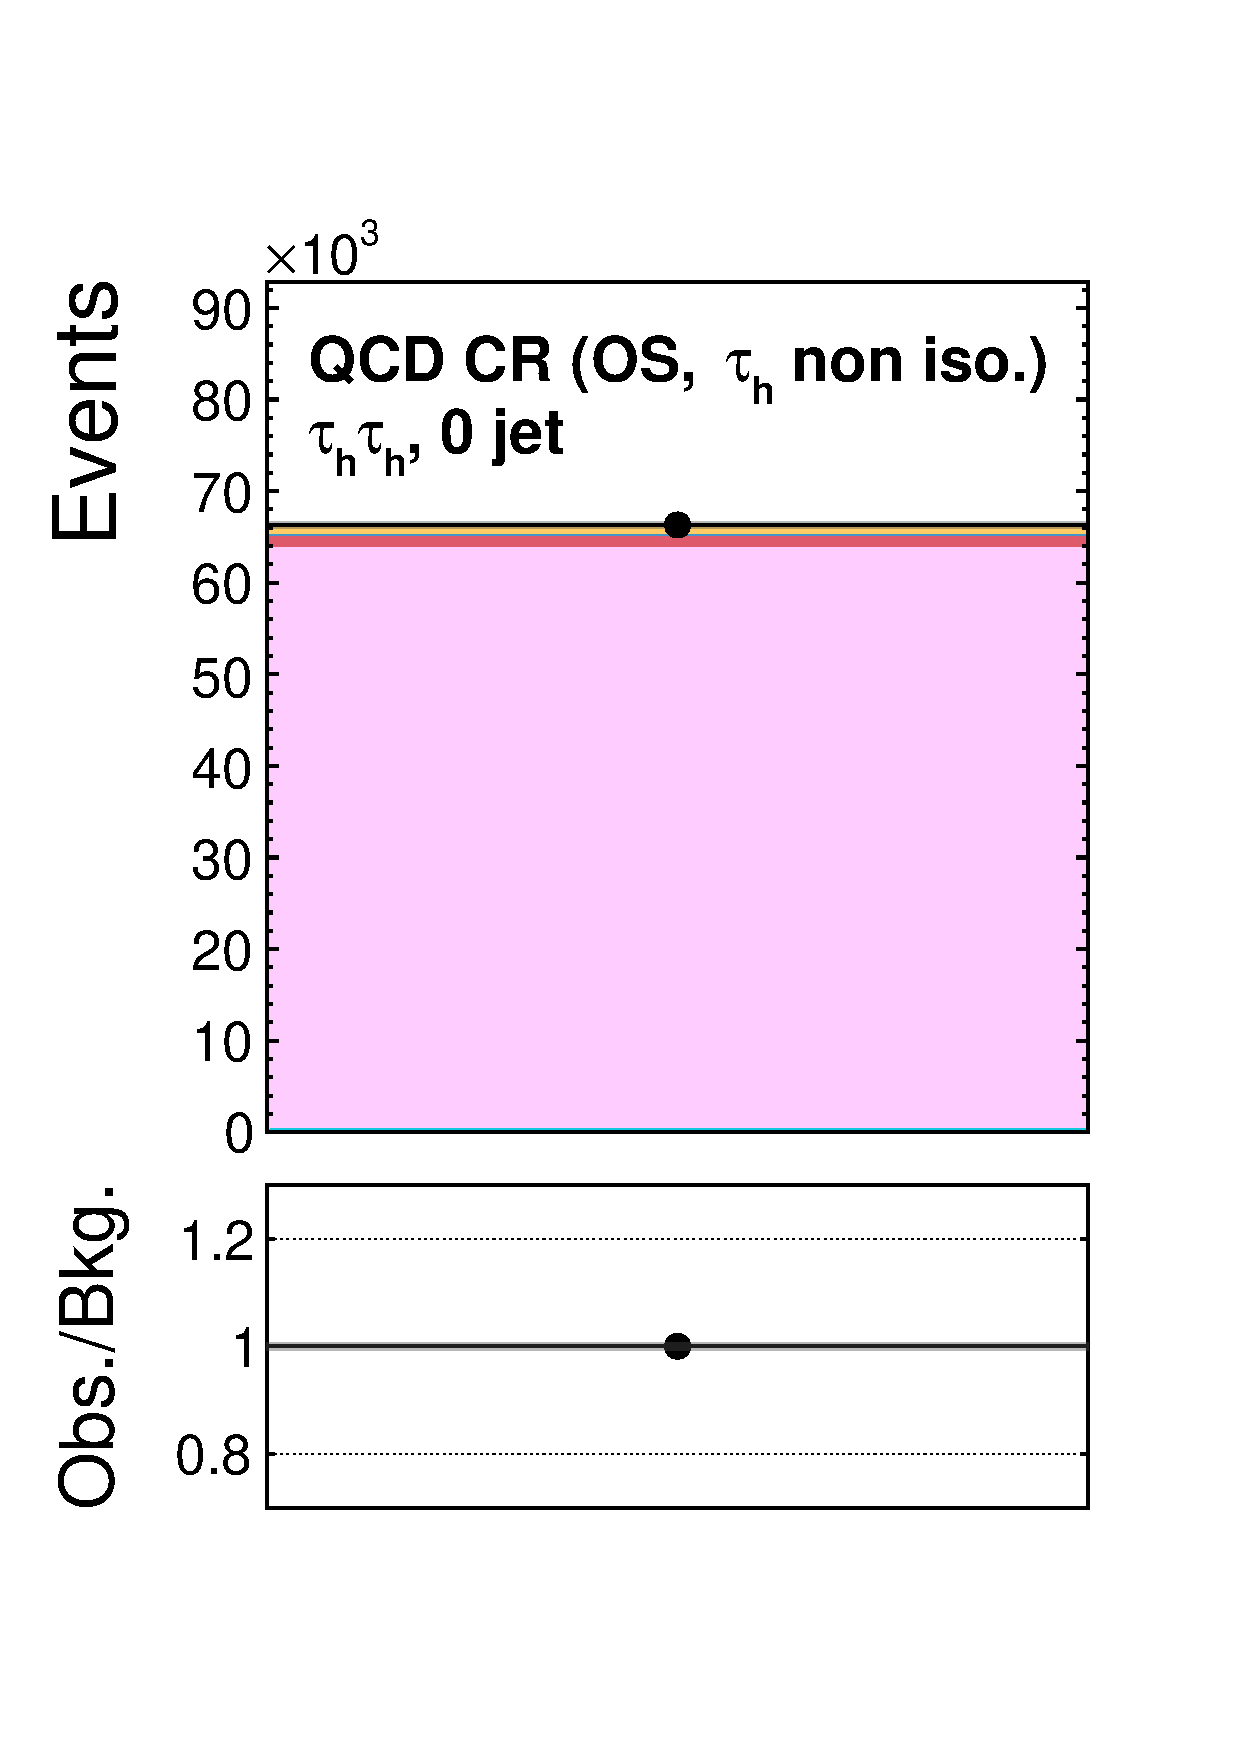
\includegraphics[width=0.24\textwidth]{figures/Figure_004-a.pdf}
     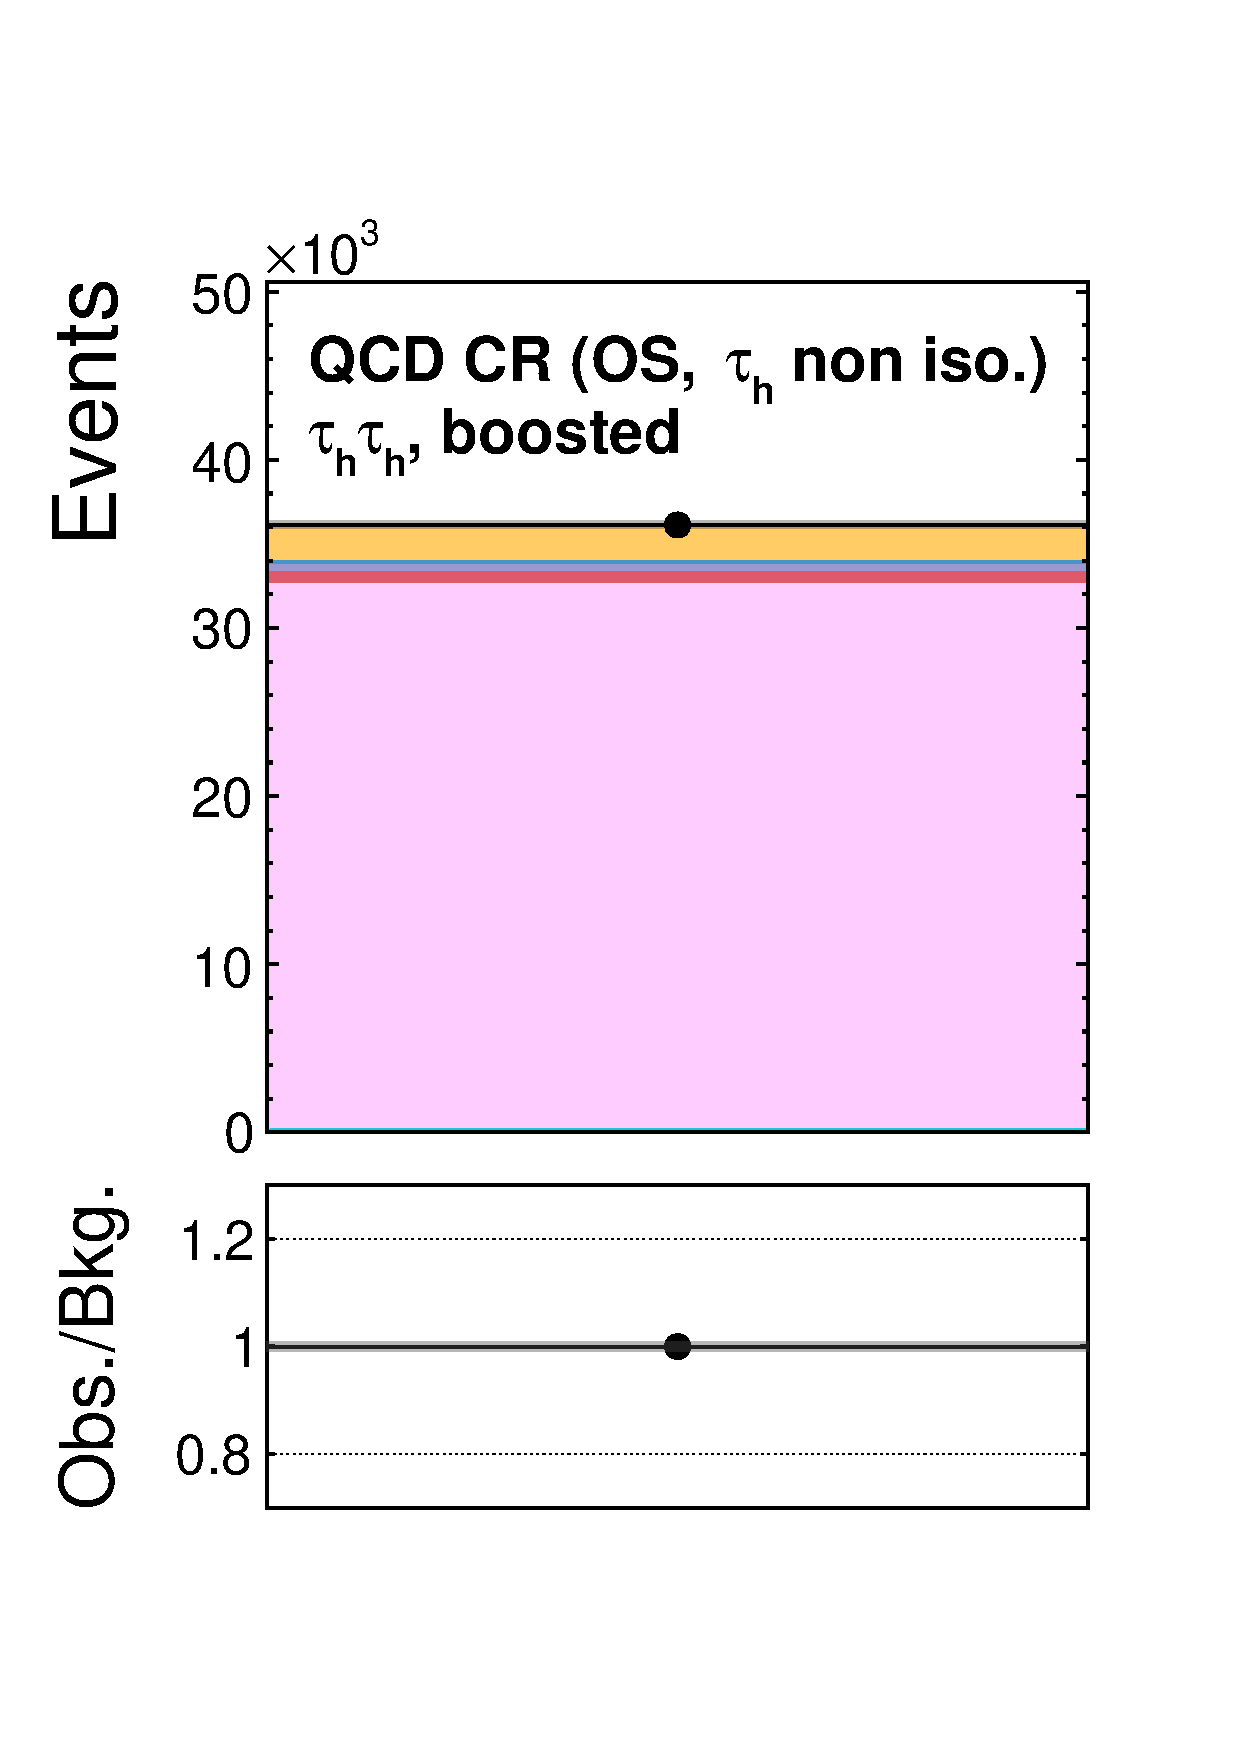
\includegraphics[width=0.24\textwidth]{figures/Figure_004-b.pdf}
     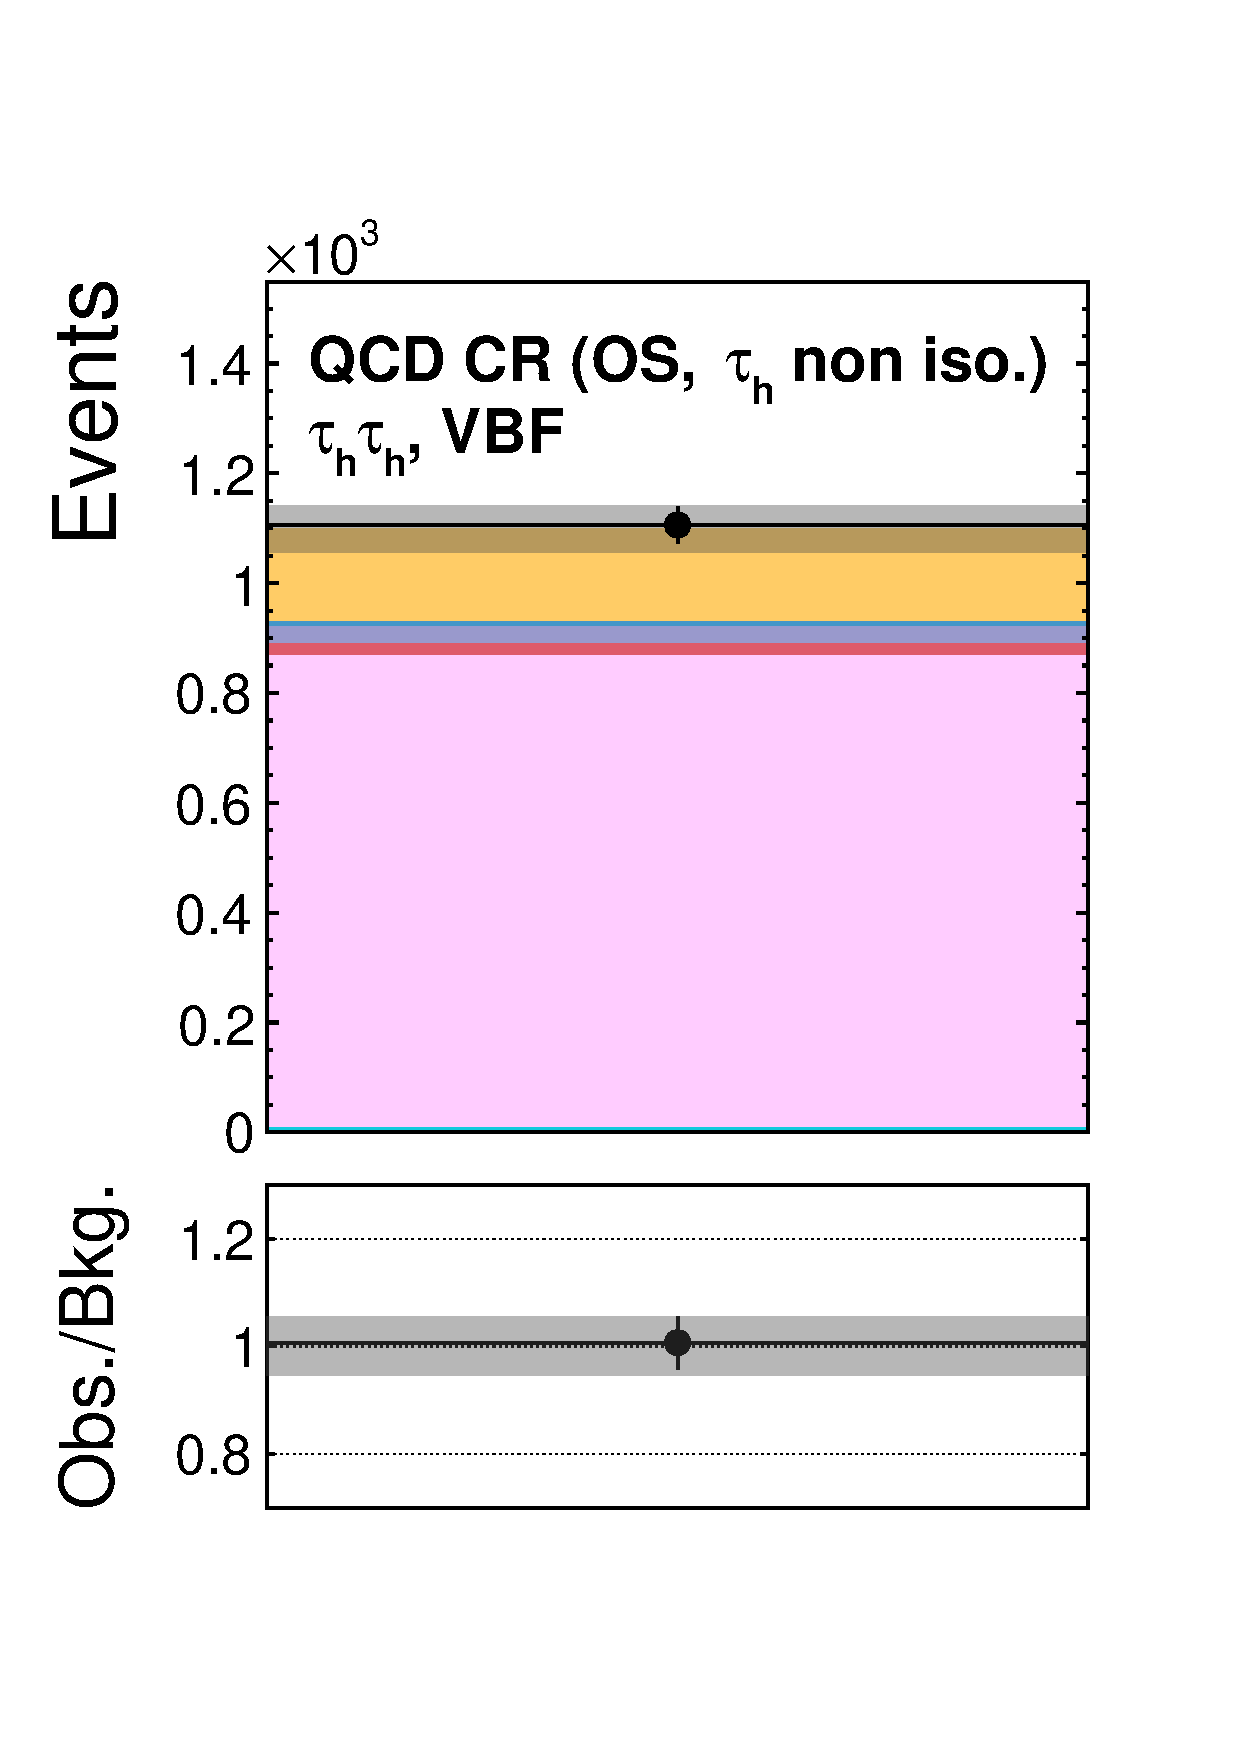
\includegraphics[width=0.24\textwidth]{figures/Figure_004-c.pdf}
     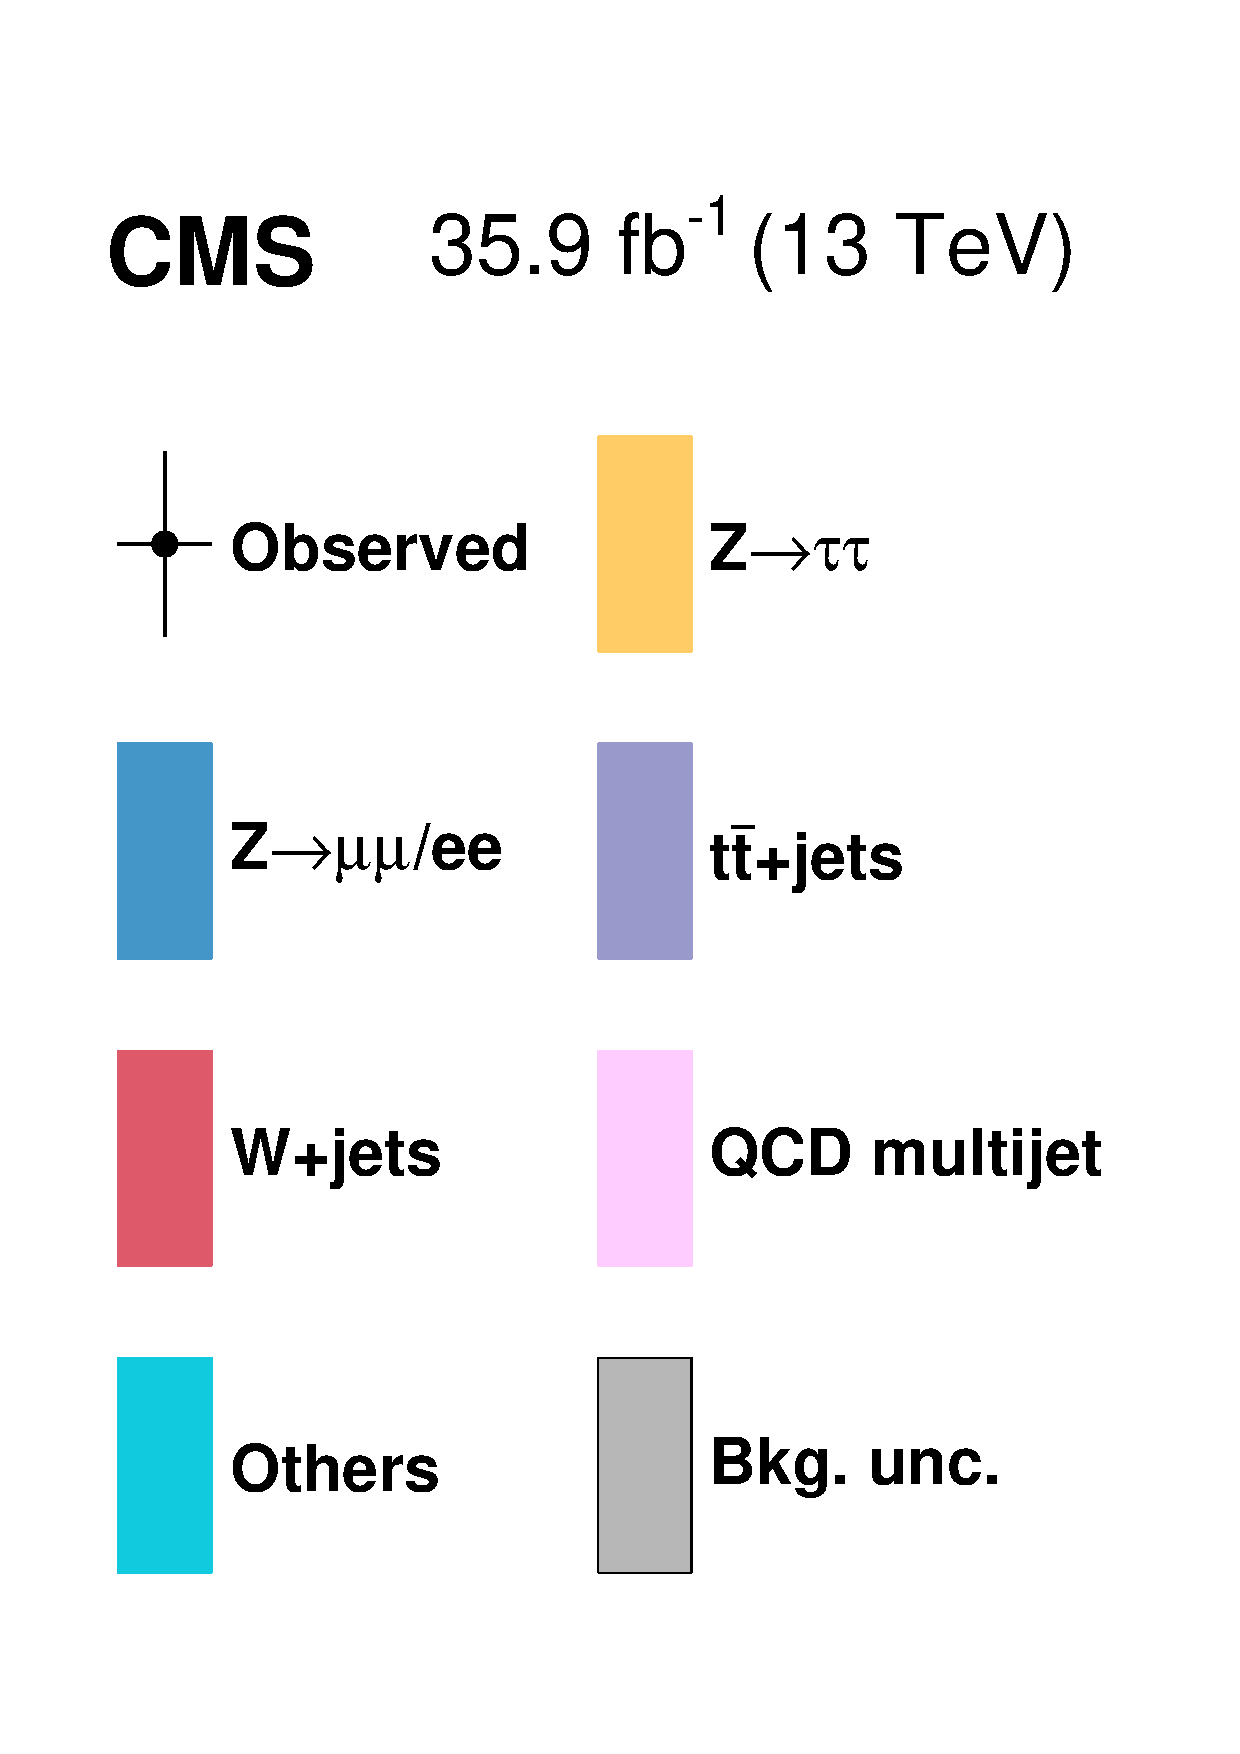
\includegraphics[width=0.24\textwidth]{figures/Figure_004-d.pdf}
     \caption{Control regions enriched in the QCD multijet background used in the maximum likelihood fit, together with the signal regions, to extract the results. The normalization of the predicted background distributions corresponds to the result of the global fit. These regions, formed by selecting events with opposite-sign $\tauh$ candidates passing relaxed isolation requirements, control the yields of the QCD multijet background in the $\tauh\tauh$ channel.}
     \label{fig:CR4}
\end{figure*}

The \ttbar production process is one of the main backgrounds in the $\Pe\Pgm$ channel.
The 2D distributions in all decay channels are predicted by simulation. The normalization is
adjusted to the one observed in a \ttbar-enriched sample orthogonal to the signal region. This control
region, shown in Fig.~\ref{fig:CR2},
is added to the global fit to extract the results, and is defined similarly as the $\Pe\Pgm$ signal region, except that the $p_\zeta$ requirement
is inverted and the events should contain at least one jet.

\begin{figure}[htb]
\centering
     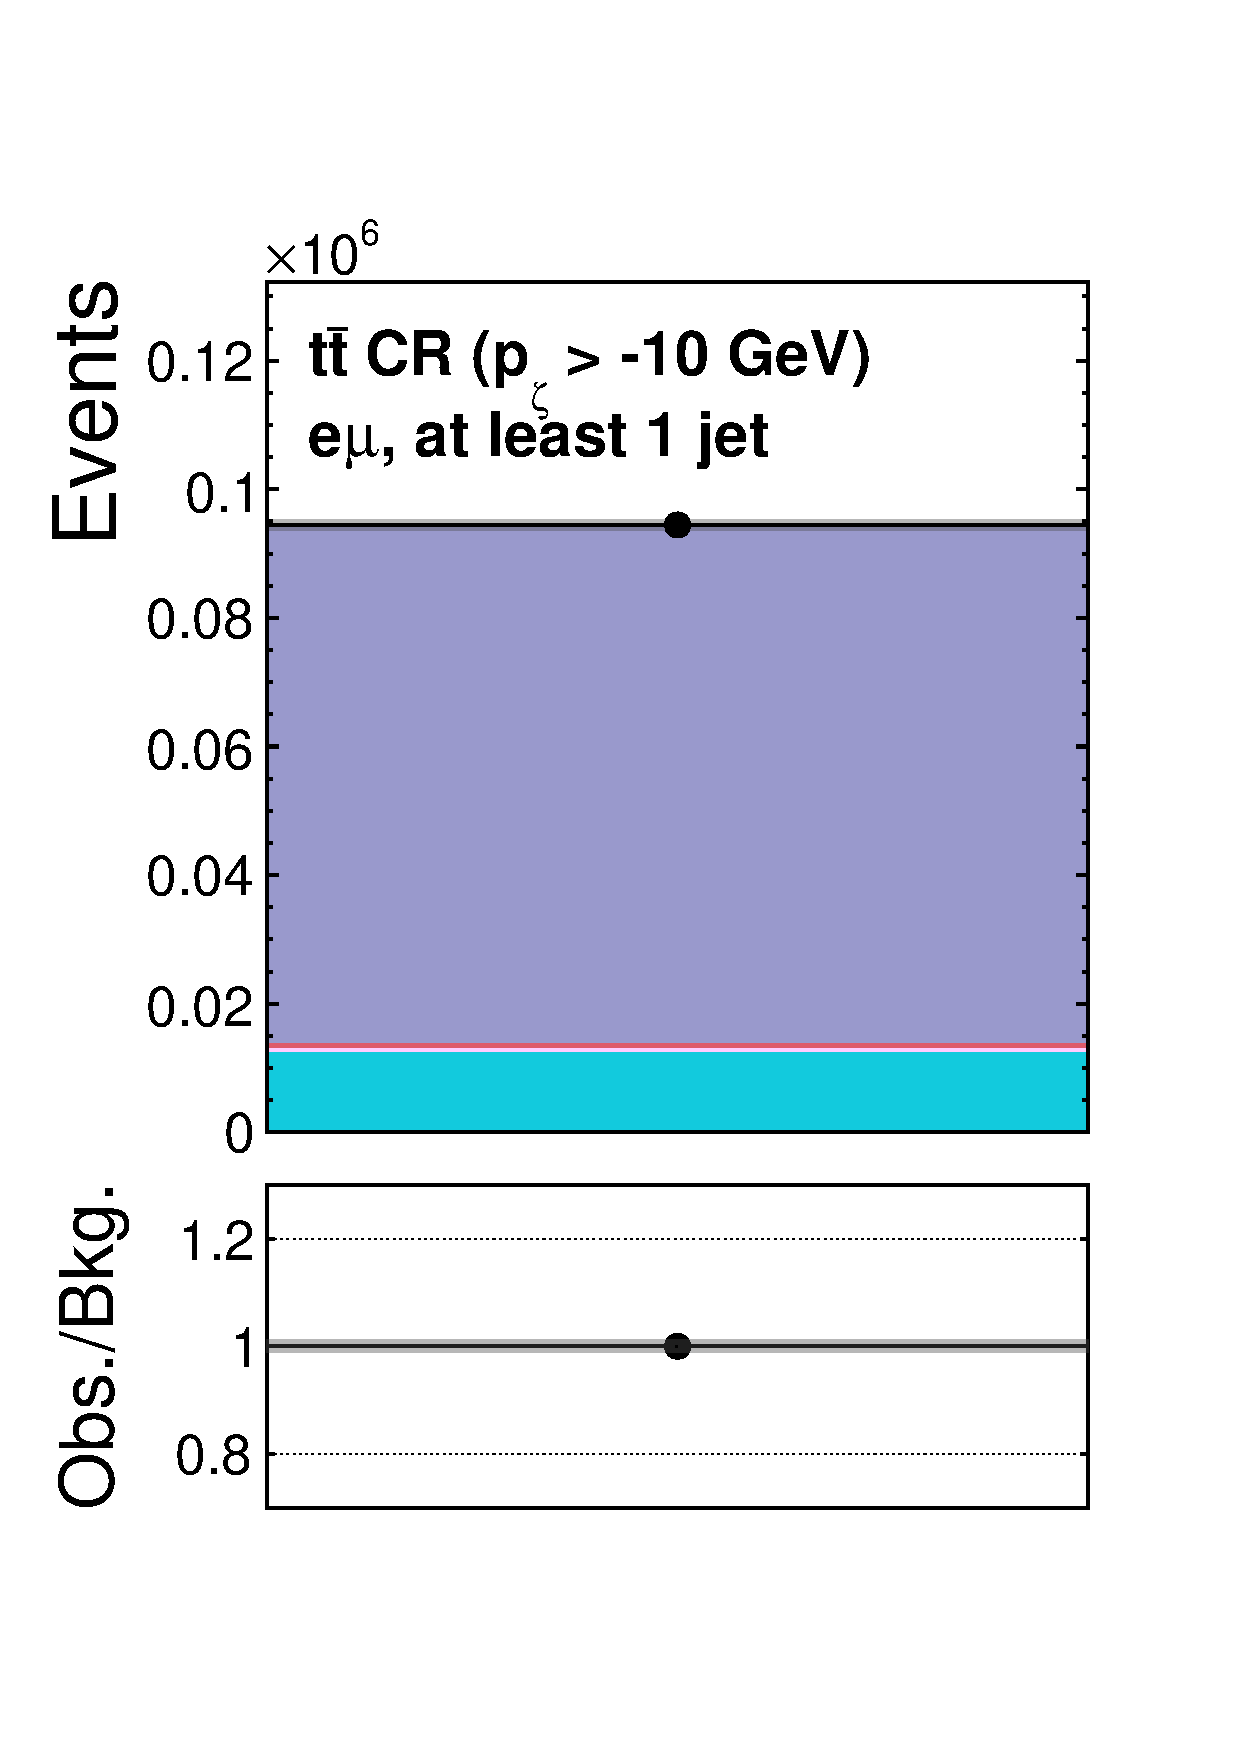
\includegraphics[width=0.23\textwidth]{figures/Figure_005-a.pdf}
     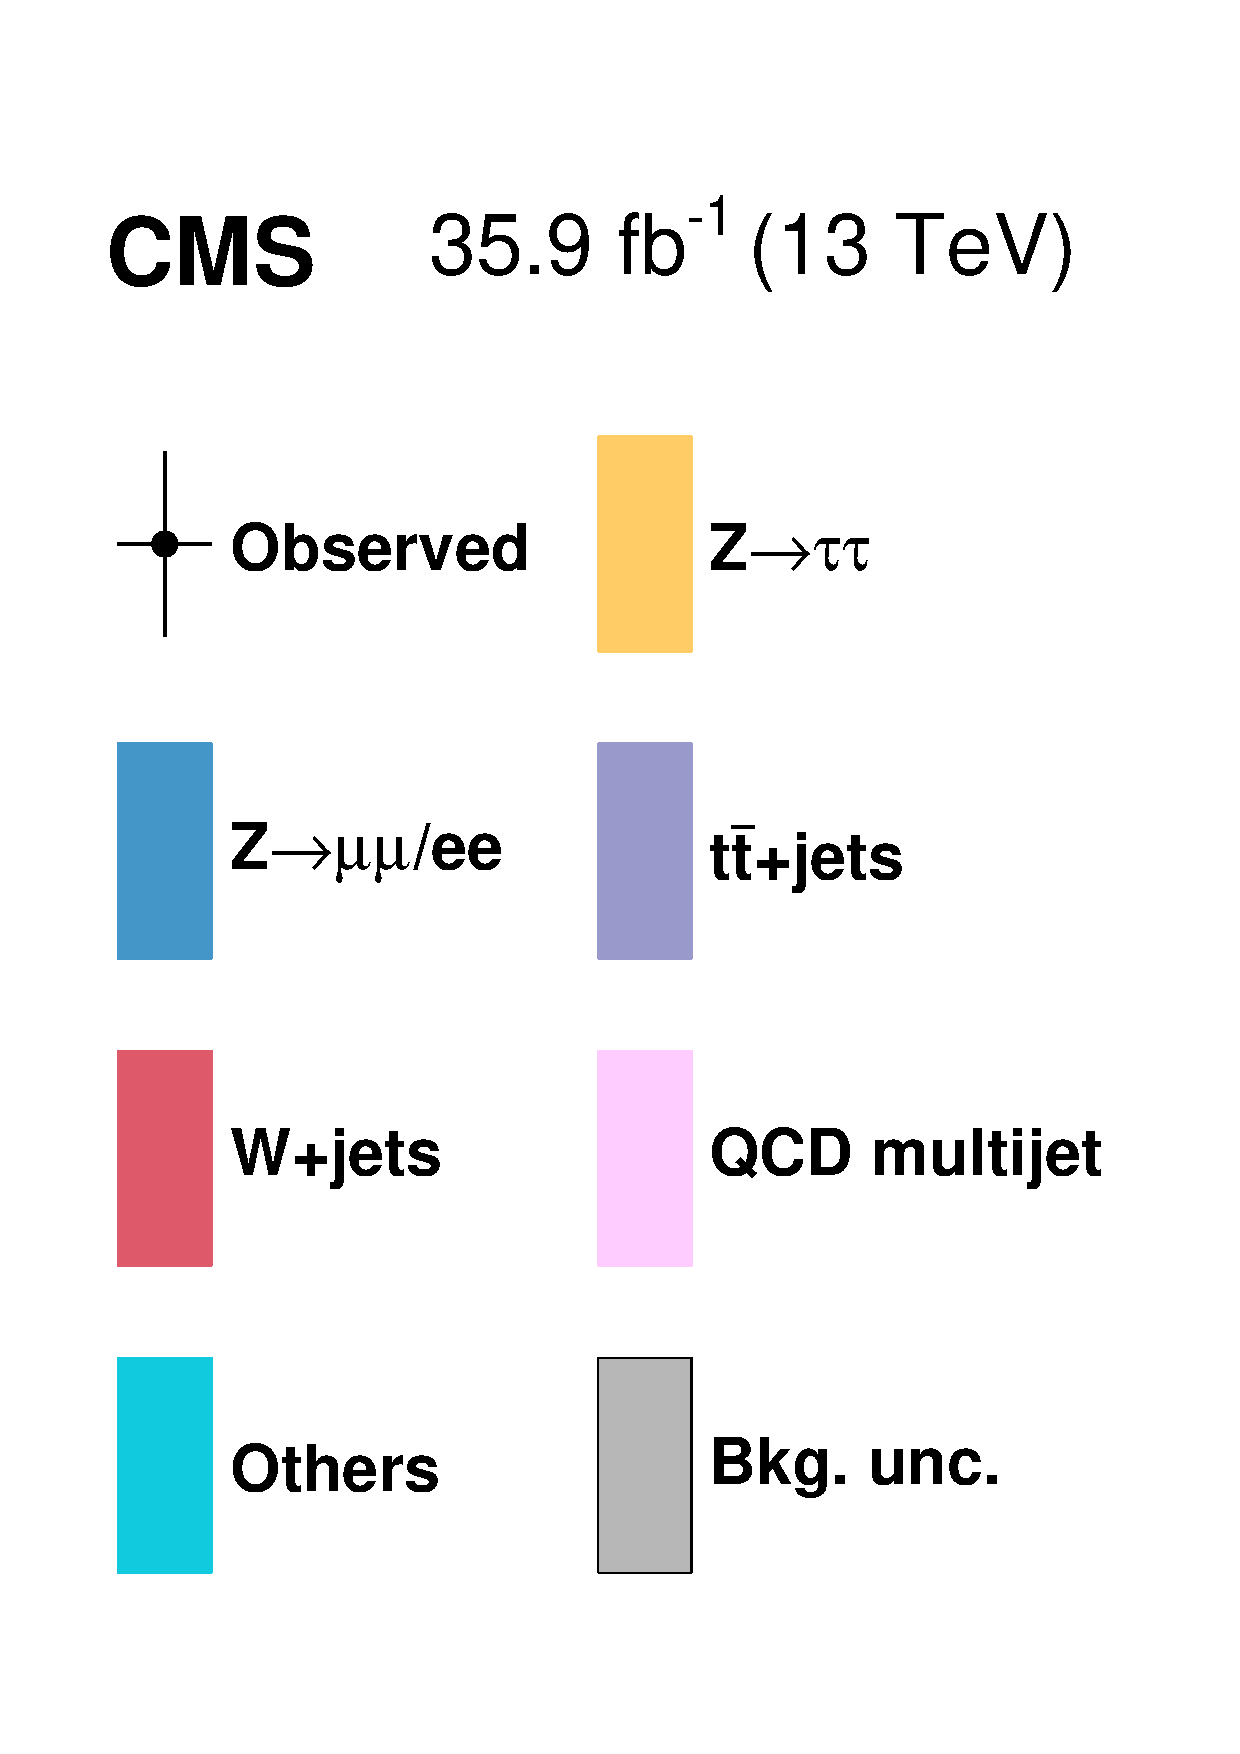
\includegraphics[width=0.23\textwidth]{figures/Figure_005-b.pdf}
     \caption{Control region enriched in the $\ttbar$ background, used in the maximum likelihood fit, together with the signal regions, to extract the results. The normalization of the predicted background distributions corresponds to the result of the global fit. This region, defined by inverting the $p_\zeta$ requirement and rejecting events with no jet in the $\Pe\Pgm$ final state,  is used to estimate the
yields of the $\ttbar$ background in all channels.}
     \label{fig:CR2}
\end{figure}

The contributions from diboson and single top quark production are estimated from simulation, as is the $\hww$ background.

\pagebreak

\section{MC Corrections}
\subsection{Pileup Reweighting}
\subsection{Tau ID Efficiency}
\subsection{Lepton ID and Isolation}
\subsection{Trigger Efficiencies}
\subsection{Recoil Corrections}
\subsection{Reweighting Drell-Yan to Data}
\subsection{Tau Energy Correction}
\subsection{Generator Event Weights}
\subsection{Luminosity}

\pagebreak

\section{Systematic Uncertainties}

\subsection{Uncertainties related to object reconstruction and identification}

The overall uncertainty in the $\tauh$ identification efficiency for genuine $\tauh$ leptons is 5\%, which has been measured with a tag-and-probe method in $\PZ\to\Pgt\Pgt$ events.
This number is not fully correlated among the di-$\Pgt$ channels because the $\tauh$ candidates are required to pass
different working points of the discriminators that reduce the misidentification rate of electrons and muons as $\tauh$ candidates.
The trigger efficiency uncertainty per $\tauh$ candidate amounts to an additional 5\%, which leads to a total trigger uncertainty of 10\% for processes estimated from simulation in the $\tauh\tauh$ decay channel. This uncertainty has also been measured with a tag-and-probe method in $\PZ\to\Pgt\Pgt$ events.

An uncertainty of 1.2\% in the visible energy scale of genuine $\tauh$ leptons affects both the distributions and the
signal and background yields. It is uncorrelated among the 1-prong, 1-prong + $\PGpz$, and
3-prong decay modes.
The magnitude of the uncertainty was determined in $\PZ\to\Pgt\Pgt$ events with one $\Pgt$ lepton decaying hadronically and the other one to a muon, by performing maximum likelihood fits for different values of the visible energy scale of genuine $\tauh$ leptons. Among these events, less than half overlap with the events selected in the $\Pgm\tauh$ channel of this analysis. The fit constrains the visible $\tauh$ energy scale uncertainty to about
0.3\% for all decay modes. The constraint mostly comes from highly populated regions with a high $\tauh$ purity, namely the 0-jet and boosted categories of the $\Pgm\tauh$ and $\tauh\tauh$ channels. The decrease in the size of the uncertainty is explained by the addition of two other decay channels
with $\tauh$ candidates ($\tauh\tauh$ and $\Pe\tauh$), by the higher number of events in the MC simulations, and by the finer categorization that leads to regions with a high $\PZ\to\Pgt\Pgt$ event purity.
Even in the most boosted categories, reconstructed $\tauh$ candidates typically have moderate $\pt$ ($\pt$ less than 100\GeV) and are
found in the barrel region of the detector. As tracks are well measured in the CMS detector for this range of $\pt$,
the visible energy scale of genuine $\tauh$ leptons is fully correlated for all $\tauh$ leptons reconstructed in the same decay mode, irrespective of their $\pt$ and $\eta$. The uncertainties in the visible energy scale for genuine $\tauh$ leptons together contribute an uncertainty of 5\% to the measurement of the signal strength.

In the 0-jet category of the $\Pgm\tauh$ and $\Pe\tauh$ channels, the relative contribution of $\tauh$ in a given
reconstructed decay mode is allowed to fluctuate by 3\% to account for the possibility that the reconstruction and
identification efficiencies are different for each decay mode. This uncertainty has been measured in a region enriched in $\PZ\to\Pgt\Pgt$ events with one $\Pgt$ lepton decaying hadronically and the other one decaying to a muon, by comparing the level of agreement in exclusive bins of the reconstructed $\tauh$ decay mode, after adjusting the inclusive normalization of the $\PZ\to\Pgt\Pgt$ simulation to its best-fit value. The effect of migration between the reconstructed $\tauh$ decay modes is negligible in other categories, where
all decay modes are treated together.

For events where muons or electrons are misidentified as $\tauh$ candidates, essentially $\PZ\to \Pgm\Pgm$ events in the $\Pgm\tauh$ decay channel and $Z\to \Pe\Pe$ events in the $\Pe\tauh$ decay channel, the $\tauh$ identification leads to rate uncertainties of 25 and 12\%, respectively, per reconstructed $\tauh$ decay mode. Using $\mvis$ and the reconstructed $\tauh$ decay mode as the observables in the 0-jet category of the $\Pgm\tauh$ and $\Pe\tauh$ channels helps reduce the uncertainty after the signal extraction fit: the uncertainty in the rate of muons or electrons misidentified as $\tauh$ becomes of the order of 5\%. The energy scale uncertainty for muons or electrons
 misidentified as $\tauh$ candidates is 1.5 or 3\%, respectively, and is uncorrelated between reconstructed $\tauh$ decay
modes. The fit constrains these uncertainties to about one third of their initial values. For events where quark- or gluon-initiated jets are misidentified as $\tauh$ candidates, a linear uncertainty that increases by 20\% per 100\GeV in $\tauh$ $\pt$ accounts for a potential mismodeling of the jet$\to\tauh$ misidentification rate as a
function of the $\tauh$ $\pt$ in simulations. The uncertainty has been determined from a region enriched in $\PW+\text{jets}$ events, using events with a muon and a $\tauh$ candidate in the final state, characterized by a large transverse mass between the $\ptmiss$ and the muon~\cite{Khachatryan:2015dfa,CMS-PAS-TAU-16-002}.

In the decay channels with muons or electrons, the uncertainties in the muon and electron identification, isolation, and trigger efficiencies lead to the rate uncertainty of 2\% for both muons and electrons.
The uncertainty in the electron energy scale, which amounts to 2.5\% in the endcaps and 1\% in the barrel of the detector, is relevant only in the $\Pe\Pgm$ decay channel, where it affects the final distributions.
In all channels, the effect of the uncertainty in
the muon energy scale is negligible.

The uncertainties in the jet energy scale depend on the \pt and $\eta$ of the jet~\cite{CMS-JME-10-011}.
They are propagated to the computation of the number of jets, which affects the repartition of events between the 0-jet, VBF, and boosted categories, and to the computation of $\mjj$, which is one of the observables in the VBF category.

The rate uncertainty related to discarding events with a b-tagged jet in the $\Pe\Pgm$ decay channel is up to
5\% for the $\ttbar$ background. The uncertainty in the mistagging rate of gluon and light-flavor jets is negligible.

The \etvecmiss scale uncertainties~\cite{CMS-JME-12-002}, which are computed event-by-event, affect the normalization of various processes through the event selection, as well as their distributions through the propagation of these uncertainties to the di-$\Pgt$ mass $\mtt$. The \etvecmiss scale uncertainties arising from unclustered energy deposits in the detector come from four independent sources related to the tracker, ECAL, HCAL, and forward calorimeters subdetectors. Additionally, \etvecmiss scale uncertainties related to the uncertainties in the jet energy scale measurement, which lead to uncertainties in the \etvecmiss calculation, are taken into account. The combination of both sources of uncertainties in the \etvecmiss scale leads to an uncertainty of about 10\% in the measured signal strength.

\subsection{Background estimation uncertainties}

The $\PZ\to\Pgt\Pgt$ background yield and distribution are corrected based on the agreement between data and the background prediction in a control region enriched in the $\PZ\to\Pgm\Pgm$ events, as explained in Section~\ref{sec:background_estimation}.
The extrapolation uncertainty related to kinematic differences in the selections in the signal and control regions ranges between 3 and 10\%, depending
on the category. In addition, shape uncertainties related to the uncertainties in the applied corrections are considered; they reach 20\% for some ranges of $\mjj$ in the VBF category. These uncertainties arise from the different level of agreement between data and simulation in the $\PZ\to\Pgm\Pgm$ control region obtained when varying the threshold on the muon $\pt$.

The uncertainties in the $\PW+ \text{jets}$ event yield determined from the control regions in the $\Pgm\tauh$ and $\Pe\tauh$ channels account for the statistical uncertainty of the observed data, the statistical uncertainty of the $\PW+ \text{jets}$ simulated sample, and the systematic uncertainties associated with background processes in these control regions. Additionally, an uncertainty in the extrapolation  of the constraints from the high-\MT ($\MT>80\GeV$) control regions to the low-\MT ($\MT<50\GeV$) signal regions is additionally taken into account. The latter ranges from 5 to 10\%, and is obtained by comparing the \MT distributions of simulated and observed $\PZ\to\Pgm\Pgm$ events where one of the muons is removed and the \etvecmiss adjusted accordingly, to mimic $\PW+\text{jets}$ events. The reconstructed invariant mass of the parent boson in the rest frame is multiplied by the ratio of the $\PW$ and $\PZ$ boson masses before removing the muon.
In the $\tauh\tauh$ and $\Pe\Pgm$ channels, where the $\PW+\text{jets}$ background is estimated from simulation, the uncertainty in the yield of this small background is equal to 4 and 20\%, respectively. The larger value for the $\Pe\Pgm$ channel includes uncertainties in the misidentification rates of jets as electrons and muons, whereas the uncertainty in the misidentification rate of jets as $\tauh$ candidates in the $\tauh\tauh$ channel is accounted for by the linear uncertainty as a function of the $\tauh$ $\pt$ described earlier.

The uncertainty in the QCD multijet background yield in the $\Pe\Pgm$ decay channel ranges from 10 to 20\%, depending on the category. It corresponds to the
uncertainty in the extrapolation factor from the same-sign to opposite-sign region, measured in events with anti-isolated leptons.
In the $\Pgm\tauh$ and $\Pe\tauh$ decay channels, uncertainties from the fit of the control regions with leptons passing relaxed isolation conditions are
considered, together with an additional 20\% uncertainty that accounts for the extrapolation from the relaxed-isolation control region to the isolated signal region.
In the $\tauh\tauh$ decay channel, the uncertainty in the QCD mutlijet background yield is a combination of the uncertainties obtained from fitting the dedicated control regions with $\tauh$ candidates passing relaxed isolation criteria, and of extrapolation uncertainties to the signal region ranging from 3 to 15\% and accounting for limited disagreement between prediction and data in signal-free regions with various loose isolation criteria.

The yield of events in a $\ttbar$-enriched region is added to the maximum likelihood fit to control the normalization of this process
in the signal region, as explained in Section~\ref{sec:background_estimation}. The uncertainty from the fit in the control region is automatically propagated to the signal regions, resulting in an uncertainty of about 5\% on the $\ttbar$ cross section. Per-channel uncertainties related to the object reconstruction and identification are considered when extrapolating from the $\Pe\Pgm$ final state to the others. The $\ttbar$ simulation is corrected for differences in the top quark $\pt$ distributions observed between data and simulation, and an uncertainty in the correction is taken into account.

The combined systematic uncertainty in the background yield arising from diboson and single top quark production processes is estimated to be 5\%
on the basis of recent CMS measurements~\cite{Khachatryan:2016tgp,Sirunyan:2016cdg}.


\subsection{Signal prediction uncertainties}

The rate and acceptance uncertainties for the signal processes related to the theoretical calculations are due to uncertainties in the PDFs, variations of the QCD renormalization and factorization scales,
and uncertainties in the modelling of parton showers.
The magnitude of the rate uncertainty depends on the production process and on the event category.

The inclusive uncertainty related to the PDFs amounts to 3.2, 2.1, 1.9, and 1.6\%, respectively, for the $ \cPg\cPg\PH $, VBF, $\PW\PH$, and $\PZ\PH$ production modes~\cite{deFlorian:2016spz}. The
corresponding uncertainty for the variation of the renormalization and factorization scales is 3.9, 0.4, 0.7, and 3.8\%, respectively~\cite{deFlorian:2016spz}.
The acceptance uncertainties related to the particular selection criteria used in this analysis are less than 1\% for the $ \cPg\cPg\PH $ and VBF productions for the PDF
uncertainties. The acceptance uncertainties for the VBF production in the renormalization and factorization scale uncertainties are also less than 1\%, while the corresponding uncertainties for the $ \cPg\cPg\PH $ process are treated as shape uncertainties as the uncertainty increases
linearly with $\pth$ and $\mjj$.

The \pt distribution of the Higgs boson in the {\POWHEG2.0} simulations is tuned to match more closely
the next-to-NLO (NNLO) plus
next-to-next-to-leading-logarithmic (NNLL) prediction in the
\textsc{HRes2.1} generator~\cite{deFlorian:2012mx,Grazzini:2013mca}.
The acceptance changes with the variation of the parton shower tune in \HERWIG++ 2.6 samples~\cite{Bellm:2013hwb} are considered as additional uncertainties, and amount to up to 7\% in the boosted category. The theoretical uncertainty in the branching fraction of the Higgs boson to $\Pgt$ leptons is equal to 2.1\%~\cite{deFlorian:2016spz}.

The theoretical uncertainties in the signal production depend on the jet multiplicity; this effect is included by following the prescriptions in Ref.~\cite{Stewart:2011cf}. This effect needs to be taken into account because the definitions of the three categories used in the analysis are based partially on the number of reconstructed jets. Additional uncertainties for boosted Higgs bosons, related to the treatment of the top quark mass in the calculations, are considered for signal events with $\pth>150\GeV$.

Theory uncertainties in the signal prediction contribute an uncertainty of 10\% to the measurement of the signal strength.





\subsection{Other uncertainties}

The uncertainty in the integrated luminosity amounts to 2.5\%~\cite{CMS-PAS-LUM-17-001}.

Uncertainties related to the finite number of simulated events, or to the limited number of events in data control regions, are taken into account. They are considered for all bins of the distributions used to extract the results if the uncertainty is larger than 5\%. They are uncorrelated across different samples, and across bins of a single distribution. Taken together, they contribute an uncertainty of about 12\% to the signal strength measurement, coming essentially from the VBF category, where the background templates are less
populated than in the other categories.

The systematic uncertainties considered in the analysis are summarized in Table~\ref{tab:uncertainties}.

\begin{table*}[!ht]
\centering
\newcolumntype{x}{D{,}{\text{--}}{2.2}}
\begin{small}
\begin{tabular}{llx}
Source of uncertainty & Prefit & \multicolumn{1}{c}{Postfit (\%) }\\
\hline
 $\tauh$ energy scale                & 1.2\% in energy scale & 0.2,0.3 \\
 $\Pe$ energy scale               & 1--2.5\%  in energy scale & 0.2,0.5\\
 $\Pe$ misidentified as $\tauh$ energy scale & 3\% in energy scale & 0.6,0.8 \\
 $\Pgm$ misidentified as $\tauh$ energy scale & 1.5\% in energy scale &  0.3,1.0\\
 Jet energy scale               & Dependent upon $\pt$ and $\eta$ & \multicolumn{1}{c}{\NA} \\
 \etvecmiss energy scale              & Dependent upon $\pt$ and $\eta$ & \multicolumn{1}{c}{\NA}  \\[\cmsTabSkip]
 $\tauh$ ID \& isolation & 5\% per $\tauh$ & \multicolumn{1}{c}{3.5} \\
 $\tauh$ trigger & 5\% per $\tauh$ & \multicolumn{1}{c}{3} \\
 $\tauh$ reconstruction per decay mode & 3\% migration between decay modes & \multicolumn{1}{c}{2} \\
 $\Pe$ ID \& isolation \& trigger  &   2\% & \multicolumn{1}{c}{\NA} \\
 $\Pgm$ ID \& isolation \& trigger & 2\% & \multicolumn{1}{c}{\NA} \\
 $\Pe$ misidentified as $\tauh$ rate   & 12\%  & \multicolumn{1}{c}{5} \\
 $\Pgm$ misidentified as $\tauh$ rate  & 25\%  & 3,8 \\
 Jet misidentified as $\tauh$ rate     & 20\% per 100\GeV $\tauh$ $\pt$ & \multicolumn{1}{c}{15}  \\[\cmsTabSkip]
 $\PZ\to\Pgt\Pgt/\ell\ell$ estimation & Normalization: 7--15\% & 3,15 \\
                             & Uncertainty in $m_{\ell\ell/\Pgt\Pgt}$, $\pt(\ell\ell/\Pgt\Pgt)$,  & \multicolumn{1}{c}{\NA} \\
                             & and $\mjj$ corrections & \\[\cmsTabSkip]
 $\PW+ \text{jets}$ estimation & Normalization ($\Pe\Pgm$, $\tauh\tauh$): 4--20\% &  \multicolumn{1}{c}{\NA} \\
                               & Unc. from CR ($\Pe\tauh$, $\Pgm\tauh$): $\simeq$5--15& \multicolumn{1}{c}{\NA} \\
                               & Extrap. from high-$m_T$ CR ($\Pe\tauh$, $\Pgm\tauh$): 5--10\% & \multicolumn{1}{c}{\NA}  \\[\cmsTabSkip]
QCD multijet estimation        & Normalization ($\Pe\Pgm$): 10--20\% & 5,20\% \\
                               & Unc. from CR ($\Pe\tauh$, $\tauh\tauh$, $\Pgm\tauh$): $\simeq$5--15\% & \multicolumn{1}{c}{\NA} \\
                               & Extrap. from anti-iso. CR ($\Pe\tauh$, $\Pgm\tauh$): 20\% & 7,10 \\
                               & Extrap. from anti-iso. CR ($\tauh\tauh$): 3--15\% & 3,10 \\[\cmsTabSkip]
 Diboson normalization & 5\% & \multicolumn{1}{c}{\NA}  \\[\cmsTabSkip]
 Single top quark normalization  & 5\% & \multicolumn{1}{c}{\NA} \\[\cmsTabSkip]
 $\ttbar$ estimation & Normalization from CR: $\simeq$5\% & \multicolumn{1}{c}{\NA} \\
                     & Uncertainty on top quark $\pt$ reweighting & \multicolumn{1}{c}{\NA}  \\[\cmsTabSkip]
 Integrated luminosity     & 2.5\% & \multicolumn{1}{c}{\NA} \\
 b-tagged jet rejection ($\Pe\Pgm$) & 3.5--5.0\% & \multicolumn{1}{c}{\NA} \\
 Limited number of events                & Statistical uncertainty in individual bins & \multicolumn{1}{c}{\NA}  \\[\cmsTabSkip]
 Signal theoretical uncertainty  & Up to 20\% & \multicolumn{1}{c}{\NA} \\
\hline
\end{tabular}
\end{small}
\label{tab:uncertainties}
\caption{Sources of systematic uncertainty. If the global fit to the signal and control regions, described in the next section, significantly constrains these uncertainties, the values of the uncertainties after the global fit are indicated in the third column. The acronyms CR and ID stand for control region and identification, respectively.}
\end{table*}
\subsection{Luminsity}
\subsection{Lepton ID and Isolation}
\subsection{QCD Estimation}
\subsection{ttbar Estimation}
\subsection{Tau Take Rate}
\subsection{Energy Scales}
\subsubsection{Tau Energy Scale}
\subsubsection{Jet Energy Scale}
\subsubsection{MET Energy Scale}
\subsection{Drell-Yan Reweighting}
\subsection{Theoretical Uncertainties for Higgs Boson}



